%%%%%%%%%%%%%%%%%%%%%%%%%%%%%%%%%%%%%%%%%%%%%%%%%%%%%%%%%%%%%%%%%%%%%%%%%%%%%%%%
%\documentclass[12pt,papel,twoside]{tesis}
\documentclass[12pt,screen,twoside,pagebackref]{tesis}
%\documentclass[12pt,papel,singlespace,oneside]{tesis}
%\documentclass[12pt,papel,preprint,singlespace,oneside]{tesis}

%%%%%%%%%%%%%%%%%%%%% Paquetes extra %%%%%%%%%%%%%%%%%%%%%%%%%%%%%%%%%%%%%%%%%%%
% Por conveniencia: aqu\'{\i} puede cargar todos los paquetes y definir los comandos 
% que necesite
\usepackage{extra}
\usepackage{enumerate}
\usepackage{algorithm}
\usepackage{algorithmic}

%%%%%%%%%%%%%%%%%%%%%%%%%%%%%%%%%%%%%%%%%%%%%%%%%%%%%%%%%%%%%%%%%%%%%%%%%%%%%%%%
%%%%%%%%%%%%%%%%%%%%% Informacion sobre la tesis %%%%%%%%%%%%%%%%%%%%%%%%%%%%%%%
\title{Software para medici\'{o}n de erosi\'{o}n y sedimentaci\'{o}n en modelos f\'{i}sicos por medio de relevamiento digital de superficies}
\author{Emanuel Sanchez Aimar}
\director{Mgs. Ing. Mariana Pagot}
\codirector{Dr. Oscar Bustos}
\carrera{Licenciatura en Ciencias de la Computaci\'{o}n}
\laboratorio{}
\grado{}
\palabrasclave{A definir}
\keywords{to define}
% Si queremos poner la fecha manualmente:
% \date{Diciembre de 2099}

%%%%%%%%%%%%%%%%%%%%%%%%%%%%%%%%%%%%%%%%%%%%%%%%%%%%%%%%%%%%%%%%%%%%%%%%%%%%%%%%
%\titlepagefalse % Si no quiere compilar la portada descomente esta linea
%\includeonly{apendices} % Compilar s\'{o}lo estos archivos 
\graphicspath{{figs/}} % Lugar donde encontrar las figuras generales (se puede poner uno en cada cap{\'{\i}}tulo)
%%%%%%%%%%%%%%%%%%%%%%%%%%%%%%%%%%%%%%%%%%%%%%%%%%%%%%%%%%%%%%%%%%%%%%%%%%%%%%%%


\begin{document}

% Dentro del environment 'preliminary' va:
% la dedicatoria, resumen, abstract, indices

\begin{preliminary}

% Escriba su dedicatoria
\dedicatoria{
A mi familia\\
A mis amigos\\
A todos los que me conocen\\
A toda esa otra gente que no
}

%%% \'{I}ndices %%%%
\tableofcontents                %\'{I}ndice
% \begin{abreviaturas}
% \end{abreviaturas}
\listoffigures                  %Figuras
% \listoftables                   %Tablas

\begin{resumen}

El presente trabajo plantea el desarrollo de una técnica experimental que permite medir la erosión y sedimentación en modelos físicos a escala reducida en laboratorio mediante la generación automática de un mapa 3D que representa la condición resultante de un ensayo hidráulico, utilizando una cámara RGB-D Microsoft Kinect. \\
Esta técnica se presenta ante la necesidad de realizar un relevamiento de erosión de un modo más preciso y eficiente respecto de la técnica utilizada tradicionalmente, que consiste en un relevamiento manual de puntos, generalmente haciendo uso de un nivel óptico y una mira milimétrica.\\ 
La técnica propuesta exhibe varios aspectos que superan al enfoque tradicional. En primer lugar, es una solución no intrusiva, es decir, no produce alteraciones sobre la condición del modelo. Además, mejora significativamente la resolución espacial del área medida, permite cubrir áreas extensas y disminuye el tiempo de medición de cada escenario ensayado. Los resultados obtenidos muestran que la solución propuesta permite realizar mediciones de erosión y sedimentación con una precisión superior a la técnica tradicional. \\

\end{resumen}

\end{preliminary}

% Podemos usar cualquiera de los dos comandos: \input o \include para incluir el texto
\chapter{Introducción}

\section{Motivaciones}
\label{S:motivaciones}

Los modelos fisicos hidraulicos son una de las principales herramientas que cuenta el campo de la Ingeniería Civil para la medición y estudio de la erosión, asi como la acumulacion y transporte de sedimentos.
Tradicionalmente, la medición de variables sedimentarias en laboratorio ha consistido en el relevamiento manual de puntos, generalmente distribuidos sobre una grilla equidistante, por medio de un nivel óptico y una mira.
Esta metodología, de carácter intrusiva (debido a que se apoya la mira sobre la superficie a relevar), presenta errores intrínsecos generados por la intervención humana y restricciones relativas a los instrumentos de medición, que pueden alcanzar los 1.5 cm. Algunas fuentes de error están relacionados con la incorrecta verticalidad de la mira, el apoyo del palpador sobre el modelo (que puede alterar la superficie a medir), errores en las lecturas y/o transcripción de las mismas, entre otros.

Por otro lado, la precisión de los productos derivados (curvas de nivel, modelos tridimensionales (3D), perfiles transversales, etc.) y los análisis de dichos productos, se verán afectados por la densidad de puntos relevados y la elección de los mismos.
Esta limitación produce un trade off entre la densidad de puntos obtenida, el área relevada y el tiempo dedicado a cada ensayo, que el ingeniero debe afrontar a la hora de realizar y completar un ensayo hidráulico fluvial en laboratorio. \\

%%% AGREGAR referencias

En el campo de la robótica, la construcción de mapas 3D del entorno físico ha sido considerado, por años, una tarea fundamental para su aplicación en la navegación autónoma y la manipulación de objetos por parte de un robot. Diferentes sensores han sido utilizados para lograr este propósito, entre ellos se puede mencionar el uso de sonares[ref], escáneres láser[ref], cámaras estereoscópicas[ref], cámaras RGB-D[ref], etc.
En los últimos años, sensores RGB-D como el dispositivo Microsoft Kinect han surgido en la industria del entretenimiento. Sus prestaciones técnicas y costo asequible lo han convertido en una solución idónea para ser utilizada en diferentes aplicaciones de Computer Vision, como es el caso de la generación de mapas 3D. \\

%%% AGREGAR : breve introducción en generacion de mapas 3D

En este trabajo se propone una nueva técnica para la medición de erosión en modelos a escala reducida mediante la generación automática de mapas 3D utilizando el sensor
RGB-D Microsoft Kinect. Esta técnica digital aplicada a procesos fluviales permite representar la superficie erosionada y/o sedimentada resultante de un ensayo hidráulico. \\
La metodología propuesta busca mejorar la caracterización obtenida del modelo físico debido a la mayor densidad de puntos obtenida. Además, busca relevar una mayor área y reducir el tiempo de medición. Esta técnica no es intrusiva, y se considera automática debido a que el único requerimiento del usuario es el desplazamiento de la cámara.

\section{Objetivos}
\label{S:objetivos}

El objetivo de este trabajo es desarrollar un software para la generación de un mapa 3D de un modelo físico a escala reducida utilizando una cámara RGB-D. Esta aplicación permitirá medir digital y automáticamente las variables de erosion y sedimentacion en laboratorio. \\
Para crear un mapa 3D del modelo, el sistema deberá capturar nubes de puntos del área de trabajo, alinearlas en un mismo sistema de coordenadas, filtrar posibles inconsistencias y realizar una conversión de escala modelo a prototipo. \\
Se validará esta nueva técnica digital con respecto a la técnica tradicional para realizar una evaluación de su precisión y verificar si es viable su aplicacion. \\
Dentro de este marco, se propone desarrollar una librería extensible y modular que permita la creación de nuevas aplicaciones, con el objetivo de aportar nuevas soluciones al problema de la medición de erosión. \\

%%% Local Variables: 
%%% mode: latex
%%% TeX-master: "template"
%%% End: 
\chapter{Revisión del estado del arte}
\label{cap:estado-del-arte}

En las áreas de robótica móvil y visión por computador, la construcción de mapas 3D del entorno ha sido tema de investigación por años. Diferentes sensores han sido utilizados con este objetivo, entre ellos, sensores laseres \cite{chou2013robotic,Montemerlo02fastslam}, camaras monoculares \cite{tomono2009robust,clemente_etal_rss2007}, camaras estereo \cite{Mei11,Konolige08}, entre otros. La mayoría de los sistemas de construcción de mapas requieren de alineación espacial entre imágenes o \textit{frames} consecutivos, detección de zonas visitadas anteriormente y alineación global de todas las imágenes para construir mapas consistentes. \\
Desde la aparición del dispositivo Microsoft Kinect (y posteriormente el Asus Xtion Pro Live \cite{asus-xtion-pro-live}) se han presentado varias soluciones al problema de construcción de mapas 3D que aprovechan tanto las características visuales como la información de profundidad que este sensor provee. En Henry et al. (2010) \cite{henry2010rgb} siguen un enfoque de extracción y emparejamiento de características visuales distintivas entre pares de frames. La información 3D asociada a estas características permite estimar la traslacion y rotacion de la cámara en un procedimiento de aproximación y refinamiento de la \textit{pose} (posicion y orientacion de la cámara) con técnicas como ICP (\textit{Iterative Closest Point}) \cite{Besl92}. En varios trabajos consultados se ha empleado este enfoque aportando modificaciones que logran mejorar su precisión y velocidad \cite{engelhard2011real,hogmanbuilding,fioraio2011realtime,6614623}. En este sentido, se cita el trabajo de Engelhard et al. (2011) \cite{engelhard2011real} en el cual se presenta un escaneo 3D de objetos y proponiendo utilizar SURF (\textit{Speed Up Robust Feateures}) \cite{bay2008speeded} a cambio de SIFT (\textit{Scale Invariant Features Transform}), empleado originalmente en \cite{henry2010rgb}, para la detección de características visuales. En Fioraio y Konolige (2011) \cite{fioraio2011realtime} plantean utilizar FAST (\textit{Features from Accelerated Segment Test})\cite{Rosten06machinelearning} y BRIEF (\textit{Binary Robust Independent Elementary Features}) \cite{Calonder12} para detectar características, y permitir la construcción de mapas 3D en tiempo real. En estas propuestas, se implementa una técnica de optimización global, conocida como SLAM (\textit{Simultaneous Localization And Mapping}) \cite{wiki-slam}, que utiliza el enfoque anterior, para detectar zonas del entorno que ya han sido visitadas, lo que permite construir mapas globalmente consistentes. \\
Por otro lado, en el centro de investigación UC Davis KeckCaves (2012) \cite{arsandbox} utilizan una cámara Kinect y un proyector digital, ambos suspendidos sobre un cajón de arena y enfocando la superficie, para crear una herramienta de realidad aumentada. La Kinect releva la superficie del cajón de arena y se proyecta un mapa digital de elevaciones (DEM, por sus siglas en inglés) en diferentes colores en tiempo real. Esta herramienta permite crear modelos topográficos, visualizar las modificaciones producidas e incluso montar simulaciones de flujo que interactúan con la información topográfica. \\
El presente trabajo se inspira en la idea propuesta en \cite{arsandbox} para medir la erosión y sedimentación de una superficie utilizando una cámara Kinect montada sobre un modelo físico hidráulico fluvial construido en el Laboratorio de Hidráulica de la facultad de Ciencias Exactas Físicas y Naturales de la UNC. Para poder relevar una superficie extensa, se aplica la solución presentada en \cite{henry2010rgb} que ha probado ser una alternativa viable para la construcción de mapas 3D. Además, se introduce SURF y ORB (Oriented FAST and Rotated BRIEF) \cite{RubleeRKB11}, propuestos por \cite{engelhard2011real} y \cite{fioraio2011realtime} respectivamente, para la detección de características visuales.


\chapter{Visión general}

Desde una perspectiva global, para generar un mapa 3D de la condición de erosión de un modelo físico utilizando una cámara RGB-D, es necesario ejecutar las siguientes etapas:
\begin{itemize}

\item Captura del frame RGB-D desde el sensor RGB-D (o desde el sistema de archivos si ya hubiesen sido grabados).

\item Registración del frame RGB-D. Se alinea el frame a un sistema de coordenadas de referencia (sistema modelo).

\item Eliminación de inconsistencias. La cámara puede relevar puntos sin información de profundidad o con mediciones incorrectas que deben ser filtrados para obtener mapas 3D consistentes. 

\item Conversión del sistema de coordenadas modelo al sistema prototipo. Inicialmente, el conjunto de frames (habiendo sido alineados o no) están en un sistema de coordenadas que tiene su origen en el sensor. Se transforma el sistema de coordenadas y se aplica el cambio de escala correspondiente (propiedad de construcción del modelo físico), a fin de obtener un modelo 3D que representa el mapa digital de elevaciones (DEM) de la condición de erosión en prototipo.

\end{itemize}

En este trabajo, la etapa de captura y registración se ejecutan incrementalmente hasta obtener un mapa 3D de la escena observada. Una vez finalizada la alineación, se realiza la eliminación de inconsistencias y finalmente se lleva a cabo la conversión a prototipo. En la figura \ref{fig:esquema-general-aplicacion} se ilustra el procedimiento implementado.
En los siguientes capítulos se explica con mayor detalle cada una de las etapas mencionadas.

\begin{figure}[ht]
\centering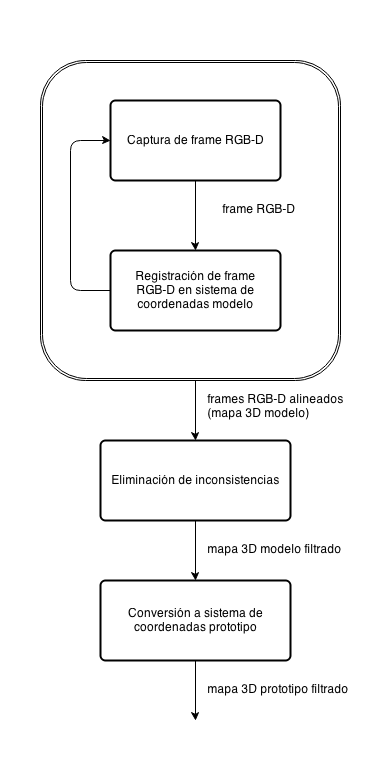
\includegraphics[width=\imsizeS]
{esquema-general-aplicacion}
\caption[Esquema general para generar mapa 3D en escala prototipo a partir de frames RGB-D.]
{Esquema general para generar mapa 3D en escala prototipo a partir de frames RGB-D.}
\label{fig:esquema-general-aplicacion}
\end{figure}



\chapter{El sensor Microsoft Kinect}

El sensor Microsoft Kinect \cite{microsoft-kinect}, inicialmente diseñado para la consola de juegos Microsoft Xbox 360 fue lanzado en Noviembre de 2010. Está compuesto por una cámara RGB (rojo, verde, azul), un sensor de profundidad, un conjunto de micrófonos y un mecanismo de inclinación motorizado. \\

\begin{figure}[ht]
\centering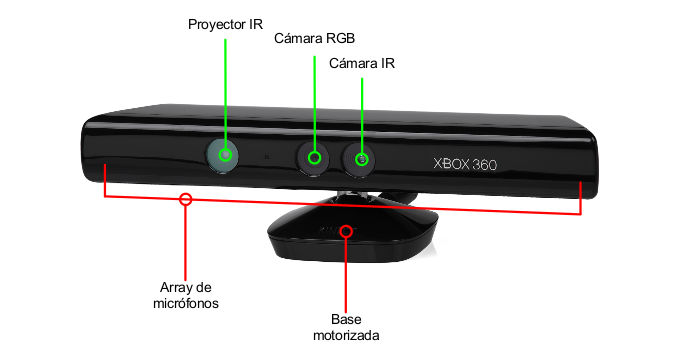
\includegraphics[width=\imsize]
{kinect}
\caption[Microsoft Kinect]
{Microsoft Kinect. Imagen original : Wikipedia bajo licencia Creative Commons\cite{wiki-kinect}.}
\label{fig:kinect}
\end{figure}

\section{Descripción}
\label{sec:descripcion-kinect}
La cámara RGB produce un \textit{stream} de datos de 24 bits por pixel, 8 bits por cada color. Su resolución estándar es 640x480 pixeles con una tasa de muestreo máxima de 30 FPS. \\
El sensor de profundidad está compuesto por un emisor láser infrarrojo (IR) y un sensor CMOS monocromo. Produce un \textit{stream} de datos de 11 bits. Posee una resolución estándar de 640x480 pixeles a una tasa de muestreo máxima de 30 FPS. \\
El campo de visión es de 57° horizontal y 43° vertical. \\
Los cámara presenta otros sensores y un mecanismo de inclinación que no fueron utilizados en este trabajo. \\

Cabe señalar que para un objeto observado en la escena, el valor de profundidad obtenido, no es la distancia real desde la Kinect al objeto, sino la distancia desde el plano del sensor (Figura \ref{fig:esquema-plano-profundidad-kinect}).

\begin{figure}[ht]
\centering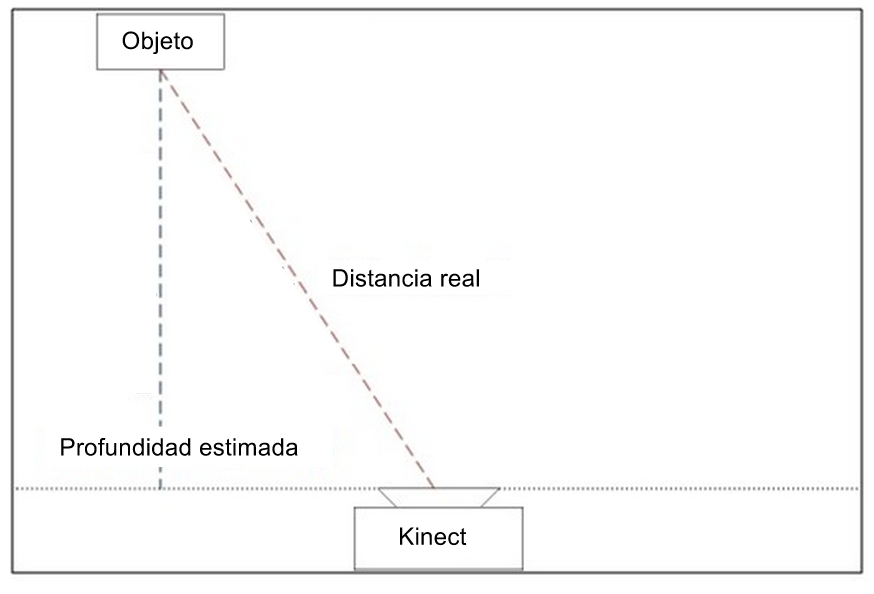
\includegraphics[width=\imsize]
{esquema-plano-profundidad-kinect}
\caption[Esquema de estimación de profundidad Kinect]
{Esquema de estimación de profundidad Kinect. Imagen original \cite{andersen12}.}
\label{fig:esquema-plano-profundidad-kinect}
\end{figure}

\section{Funcionamiento interno}
\label{sec:funcionamiento-kinect}

El funcionamiento de la cámara Kinect esta basado en tecnología propiedad de la empresa israelí PrimeSense \cite{primesense}. \\
Para obtener una imagen de profundidad el emisor láser emite un patrón de puntos que es capturado por la cámara infrarroja (sensor CMOS monocromo). Figura \ref{fig:kinect-patron-ir}. \\

\begin{figure}[ht]
\centering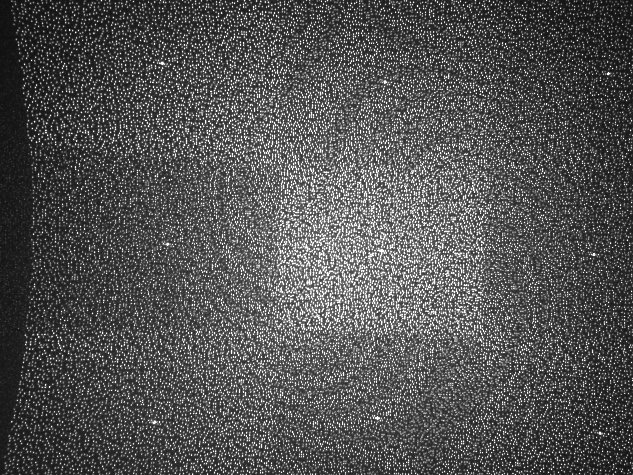
\includegraphics[width=\imsizeS]
{kinect-patron-ir}
\caption[Patrón de puntos emitido por el sensor IR]
{Patrón de puntos emitido por el sensor IR. Fuente : proyecto ROS\cite{ros} bajo licencia Creative Commons.}
\label{fig:kinect-patron-ir}
\end{figure}

El proceso que se describe en la patente de PrimeSense\cite{garcia2008range} se divide en las siguientes etapas :
\begin{enumerate}
\item Capturar el patrón de puntos para un conjunto de imágenes de referencia a diferentes distancias del plano del sensor.
\item Capturar el patrón de puntos sobre una imagen de test de la region de interes.
\item Encontrar la imagen de referencia que mayor similitud tiene con la imagen de test utilizando un método de Correlación Cruzada\cite{wiki-cross-correlation}.
\item Estimar el mapa 3D de la escena por medio de un proceso de triangulación utilizando los desplazamientos entre la imagen de test y la imagen de referencia elegida.
\end{enumerate}

En el caso del Microsoft Kinect, las imágenes de referencia han sido capturadas contra una superficie plana a distancias predefinidas y están almacenadas en el dispositivo. El sensor devuelve la imagen de profundidad en forma de valores de disparidad que luego son traducidos a distancias en metros, en un procedimiento externo, mediante la conversión :

\begin{equation}
distancia=0.1236 \cdot \tan(\frac{disparidad}{2842.5} + 1.1863)
\end{equation}

Si bien el sensor Kinect captura las imágenes RGB y de profundidad de forma independiente, en este trabajo se utiliza una librería que brinda la posibilidad de sincronizar automáticamente ambos tipos de imágenes, dando como resultado una imagen RGB-D o frame RGB-D.

\section{Consideraciones}
\label{sec:consideraciones-kinect}

En este apartado se describen algunas especificaciones para el uso del dispositivo Kinect que se consideran relevantes para este trabajo.

De acuerdo a las especificaciones oficiales, el rango de operación del sensor de profundidad se encuentra entre 0.4 m a 4 m. En Khoshelham\cite{khoshelham2011accuracy} (2011) se analiza la precisión del sensor, midiendo la profundidad de una superficie plana a diferentes distancias y se concluye que el error aleatorio de los datos de profundidad crece cuadráticamente con el aumento de la distancia entre el dispositivo y la escena observada, según se presenta en la figura \ref{fig:error-kinect}.

\begin{figure}[ht]
\centering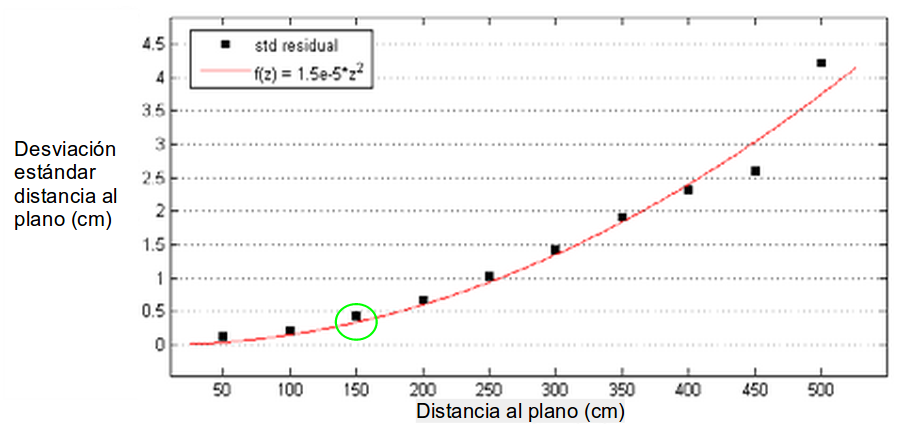
\includegraphics[width=\imsize]
{error-kinect}
\caption[Error camara Kinect]
{Desviación estándar del error en la estimación de profundidad, posicionando el sensor a diferentes distancias del plano de referencia. En rojo se muestra la curva que mejor ajusta al error. La desviación estándar presenta un valor de 0,5 cm a una distancia de 1,5 m y un maximo cercano a 4,25 cm para una distancia de 5 m. Fuente : \cite{khoshelham2011accuracy}.}
\label{fig:error-kinect}
\end{figure}

En Andersen y Ahrendt\cite{andersen12} (2012) se realiza otro análisis del sensor de profundidad del Microsoft Kinect concluyendo lo siguiente :
\begin{itemize}

\item Materiales con características reflectantes influyen sobre el sensor de profundidad imposibilitando la medición de distancias o derivando en mediciones incorrectas.

\item La luz infrarroja, en particular la luz solar, interfiere con el sensor IR limitando su utilización en entornos exteriores.

\item Debido a la distancia interna entre el emisor y el detector IR en el dispositivo Kinect, los objetos iluminados pueden provocar sombras en la imagen de fondo (Figura \ref{fig:sombra-kinect}). La sombra en el patrón imposibilita que el sensor pueda calcular la profundidad y los píxeles en el área sombreada se ponen a profundidad cero. En la figura \ref{fig:silla-sombra-kinect}, se puede observar la imagen RGB (derecha) y de profundidad (izquierda) de una silla. La cámara no pudo capturar la profundidad del borde izquierdo de silla (área en azul) debido a la posición relativa de los sensores IR con respecto a la escena.

\end{itemize}

\begin{figure}[ht]
\centering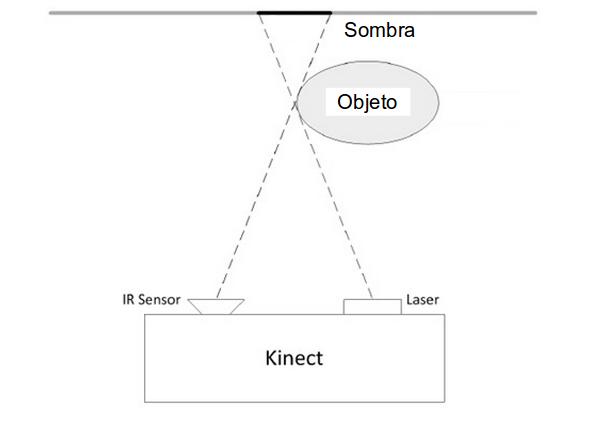
\includegraphics[width=\imsizeS]
{sombra-kinect}
\caption[Esquema de sombras en la imagen de profundidad generada por la cámara Kinect]
{Esquema de sombras en la imagen de profundidad generada por la cámara Kinect. Imagen original : \cite{andersen12}.}
\label{fig:sombra-kinect}
\end{figure}

\begin{figure}[ht]
\centering
\begin{minipage}[ht]{.45\textwidth}
\begin{center}
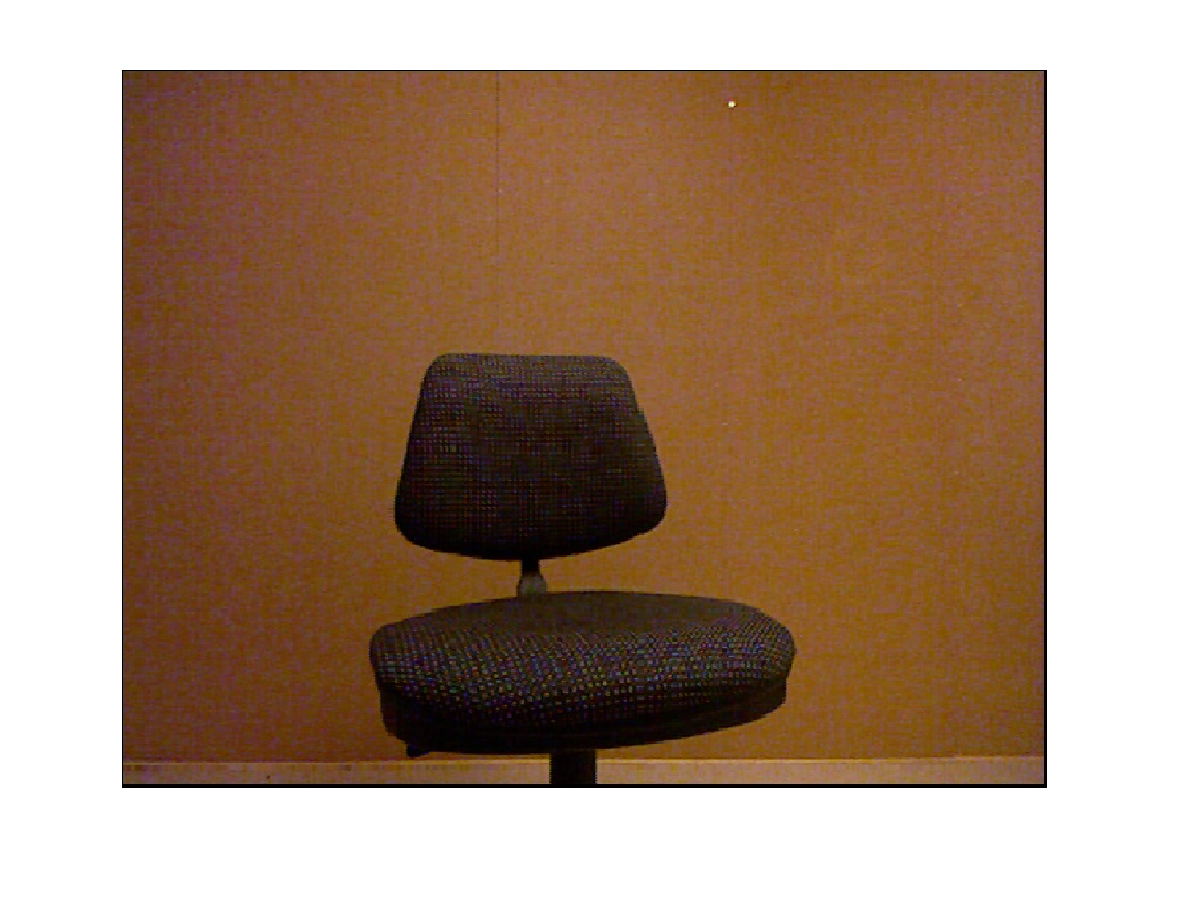
\includegraphics[width=\imsizeS]{silla-rgb-kinect}
\end{center}
\end{minipage}
\hfill
\begin{minipage}[ht]{.45\textwidth}
\begin{center}
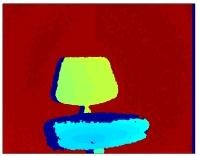
\includegraphics[width=0.91\textwidth]{silla-depth-kinect}
\end{center}
\end{minipage}
\hfill
\caption[Silla con zonas sin medición de profundidad]{Imágenes RGB (derecha) y de profundidad (izquierda) de una silla con zonas sin mediciones de profundidad (en azul). Imagen original : \cite{andersen12}.}
\label{fig:silla-sombra-kinect}
\end{figure}



\chapter{Registracion}

\section{Caracteristicas visuales}

La deteccion de caracteristicas visuales (feature en ingles) es una tecnica muy utiliza en vision por computador para la deteccion, reconocimiento y seguimiento de objetos. Hay dos tareas que deben realizarse para encontrar caracteristicas visuales : la deteccion de un punto de interes (keypoint en ingles), que identifica un area relevante en la imagen, y el computo de un descriptor, que caracteriza a la region. Por lo general, el algoritmo de deteccion identifica regiones en la que su intensidad varia mucho, por ejemplo bordes o esquinas de un objeto, y se selecciona el centro de la region como punto de interes. El descriptor suele representarse como un vector multidimensional que, por lo general, se calcula en base a metricas (como puede ser la orientacion) a partir de los puntos circundantes al keypoint. Es deseable que las caracteristicas detectadas sean invariantes a rotacion, translacion, cambios de iluminacion y escala.

% EXPLICAR PORQUE SE ELIGUEN SURF Y ORB.

\begin{subsection}
{Speeded Up Robust Feature (SURF)}

The Speeded Up Robust Feature (SURF) provides a robust detector and descrip-
tor, that can be used in computer vision tasks like object recognition or 3D
reconstruction. It is partly inspired by the SIFT descriptor, both are using local
gradient histograms. The main difference concerns the performance, lowering the
computational time through an efficient use of integral images for the image con-
volutions, Hessian matrix-based detector (optimized through approximations of the
second order Gaussian partial derivatives, see figure 2.5), and sums of approximated
2D Haar wavelet responses for the descriptor (see figure 2.7). The standard version
of SURF is several times faster than SIFT and claimed by its authors to be more
robust against different image transformations than SIFT.

SURF es un detector y descriptor de caracteristicas \cite{bay2008speeded} en parte inspirado por el descriptor SIFT CITAR[PAPER]. La principal diferencia es la velocidad, siendo la version estandar de SURF un orden magnitud mas rapido que SIFT, y segun sus autores, mas robusto ante diferente tipo de transformaciones.

\begin{subsection} 
{El detector de caracterısticas de SURF}
EL detector de SURF se base en el determinante de la matrix Hessiana. Dada una funcion continua f(x, y), la matrix Hessiana H esta formada por la derivadas parciales de f :

AGREGAR FORMULA DE H.

Siendo el determinante de esta matrix : AGREGAR FORMULA DE DET(H).
A partir del test de la segunda derivada REFERENCIAR, se tiene que si el determinante es positivo se puede clasificar a ese punto de la funcion como un maximo o minimo local, mientras que si es negativo se obtiene que no es un extremo local.

REFERENCIA
[Si la Hessiana es definida positiva en x, entonces f (x) tiene un m ́
ınimo local en x. Si la Hessiana es
definida negativa, entonces f (x) tiene un m ́
aximo local en x. Si la Hessiana tiene autovalores positivos y
negativos, f (x) es un punto de silla. En otro caso el test no aporta informaci ́
on.]

Al aplicar esta teoria al dominio de las imagenes, se sustituye f(x, y)
por la intensidad de los pixeles de la imagen I(x, y) y se reemplaza el calculo de 
las derivadas parciales por la aplicacion de filtros de convolucion. En particular, para calcular las derivadas parciales se pueden utilizar kernels que discretizan las derivadas segundas de la funcion Gaussiana, con Lxx(x, sigma) denotando la evaluacion de derivada parcial. Sin embargo, los autores de SURF proponen una aproximacion a estos kernels por medio de box filters. Como se observa en la figura, los box filters son filtros de convolucion muy simples, que pueden ser aplicados eficientemente utilizando una representacion intermedia de la imagen, la imagen integral \cite{Crow84}.

Para calcular el determinante de la Hessiana por medio de box filters se utiliza una aproximacion, denominada blob response en (x, y, sigma), que se define como : 
AGREGAR FORMULA.

Para encontrar las caracteristicas visuales se utiliza el concepto de espacio de escalas (scale space). El espacio de escalas de una imagen I es una funcion continua, parametrizada en t, que representa un conjunto (infinito) de imagenes, obtenidas a partir de suavizar I, con resultados mas pronunciados a medida que t crece. Tradicionalmente, un scale space se suele implementar como una piramide imagenes donde iterativamente se aplican filtros de suavizado por convolucion y se reduce el tamaño de la imagen. Este metodo se aplica en SIFT, pero es computacionalmente costoso debido al re-escalado de las imagenes. En SURF, se implementa un enfoque diferente, basado en el hecho que la construccion de un box filter no depende del tamaño del mismo, por lo se construye una piramide de filtros para ser utilizados con la imagen original. De esta forma, permite calcular el blob response en varias escalas en paralelo, sin necesidad de re-escalar la imagen. En la figura \ref{fig:scale-space} se ilustra la diferencia entre el enfoque aplicado en SIFT y el propuesto en SURF para la construccion del espacio de escalas.

\begin{figure}[ht]
\centering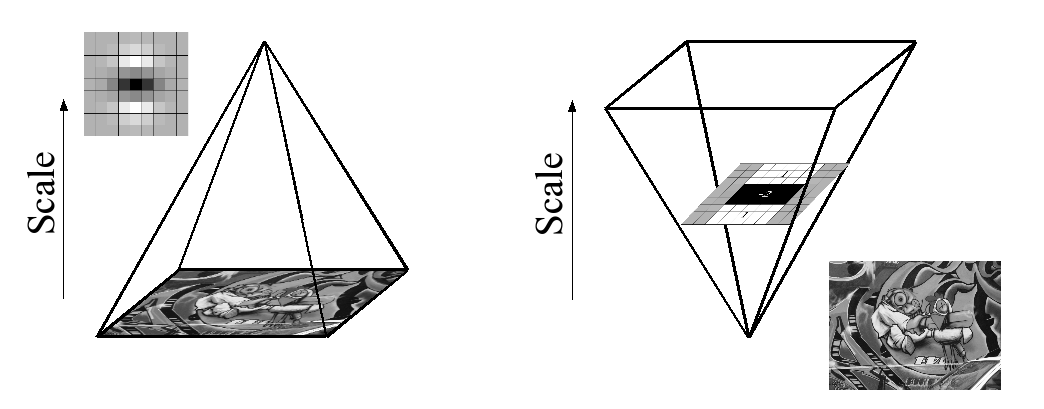
\includegraphics[width=\imsize]
{scale-space}
\caption[Espacio de escalas]
{Enfoques para construir el espacio de escalas. Izquierda : enfoque tradicional donde iterativamente se re-escala la imagen y se suaviza con un filtro Gaussiano de un determinado tamaño. Derecha : enfoque propuesto por SURF donde aplican filtros de diferente tamaño (utilizando la imagen integral) manteniendo la imagen original. Fuente : \cite{bay2008speeded}.}
\label{fig:scale-space}
\end{figure}

El proceso de deteccion SURF se divide en 3 etapas :
\begin{itemize}

\item Filtrado de blob responses : caracteristicas con respuesta por debajo de un umbral se eliminan. Incrementar el umbral reduce la cantidad de caracteristicas detectadas dejando la mas robustas. 

\item Aplicacion del algoritmo de non-maximal suppresion : se compara el pixel candidato con sus 26 vecinos (8 en la escala del candidato y 9 en las escalas superior e inferior) descartandolo cuando su respuesta no es maxima.

\item Interpolacion : se interpolan los datos en la cercania del candidato para obtener una localizacion con precision de subpixel.

\end{itemize}

\end{subsection}

\begin{subsection} 
{El descriptor de SURF}
El descriptor de SURF describe como se distribuye la intensidad de los pixeles vecinos de una caracterisitica encontrada con el detector previamente explicado. El computo del descriptor tiene 2 etapas : la extraccion de la orientacion predominante de la caracteristica y el computo de los componentes del vector utilizando Haar wavelets. \\ Los Haars wavelets son filtros que se utilizan para calcular los gradientes en x y y. Como se observa en la figura \cite{fig:haar-wavelet}, la simplidad de los filtros, permite aplicar la representacion de la imagen integral para implementar la convolucion de forma eficiente.

\begin{figure}[ht]
\centering
\begin{minipage}[h]{.45\textwidth}
\begin{center}
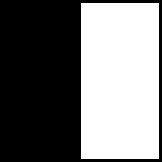
\includegraphics[width=\imsizeS]{haar-wavelet-x}
\end{center}
\end{minipage}
\hfill
\begin{minipage}[h]{.45\textwidth}
\begin{center}

\includegraphics[width=\imsizeS]{haar-wavelet-y}
\end{center}
\end{minipage}
\hfill
\caption[Haar wavelet]{Filtros Haar wavelet utilizados para computar los gradientes en la direccion x (inquierda) e y (derecha). La parte negra representa el valor −1 y la parte blanca +1. Imagen original : \cite{bay2008speeded}.}
\label{fig:haar-wavelet}
\end{figure}

Para extraer la orientacion de una feature se realizan 2 tareas : 

\begin{enumerate}

\item Se computan las respuestas Haar wavelet de tamaño 4 sigma (siendo sigma la escala asociada al punto de interes) en un radio de 6 sigma alrededor de la caracteristica, para obtener las componentes x e y del gradiente. A las respuestas obtenidas se les aplica una Gaussina (con desvicion de 2 sigma) centrada en el punto de interes. Para cada pixel del area circular, se les asocia un punto 2D en el espacio dado por el vector gradiente.

\item Seleccion de la direccion predominante de las respuestas. Se rota una ventana de tamaño pi/3 alrededor del origen de la caracteristica y se suman las componentes de las respuestas dentro de la seccion. El vector resultante con mayor modulo representa la orientacion predominante del punto de interes. El procedimiento se ilustra en la figura \ref{fig:orientacion-surf}.

\end{enumerate}

\begin{figure}[ht]
\centering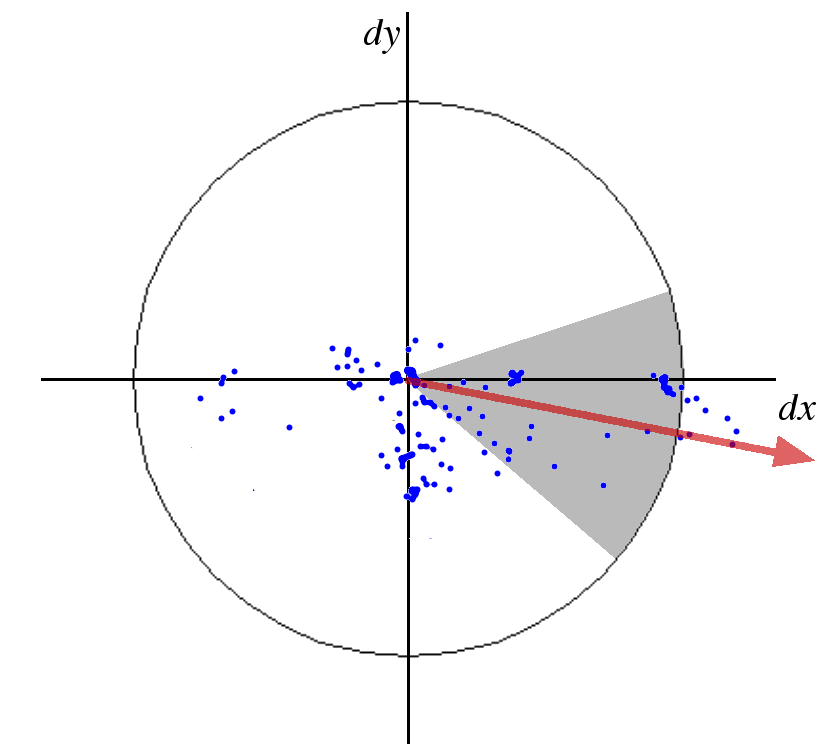
\includegraphics[width=\imsize]
{orientacion-surf}
\caption[Calculo de la orientacion para una caracteristica SURF]
{ La orientacion dominante de la caracteristica se encuentra rotando una ventana de pi/3 alrededor del keypoint, sumando las componentes de las repuestas producidas por los filtros Haar wavelets dentro de la ventana y seleccionando la orientacion del vector resultante con mayor modulo. Fuente : \cite{bay2008speeded}.}
\label{fig:orientacion-surf}
\end{figure}

En algunas aplicaciones, la invarianza de rotacion no es necesaria, lo que permite omitir este paso, dando lugar al denominado Upright SURF (U-SURF).

Para la extraccion de los componentes del descriptor SURF, el primer paso consiste en construir una region rectangular de tamaño 20 sigma alrededor de la caracteristica y orientada en la direccion predominante obtenida en la etapa anterior. La region se divide en 4x4 subregiones rectangulares, y para cada una se computa la respuesta de Haar wavelet de tamaño 2 sigma sobre 25 puntos distribuidos regularmente. Denotando dx y dy, a las respuestas en la direccion x e y respectivamente, se obtiene para cada subregion un vector de la forma v (formula). 
El descriptor resultante se compone por los vectores de cada subregion, por lo que su tamaño es 4 x 4 x 4 = 64 elementos.

\begin{figure}[ht]
\centering
\begin{minipage}[h]{.45\textwidth}
\begin{center}
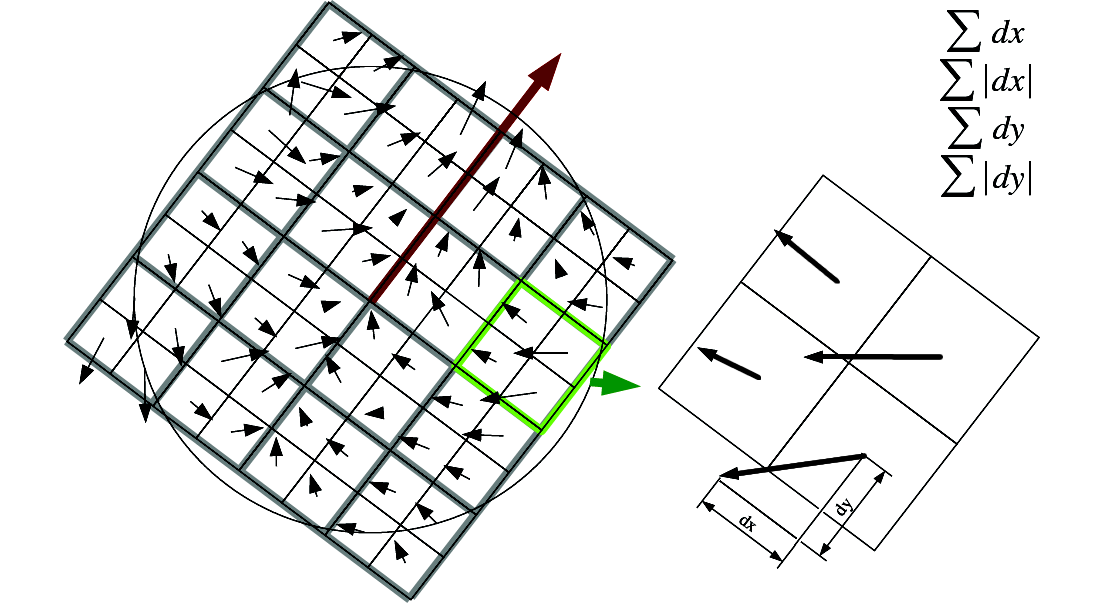
\includegraphics[width=\imsizeS]{grilla-surf}
\end{center}
\end{minipage}
\hfill
\begin{minipage}[h]{.45\textwidth}
\begin{center}
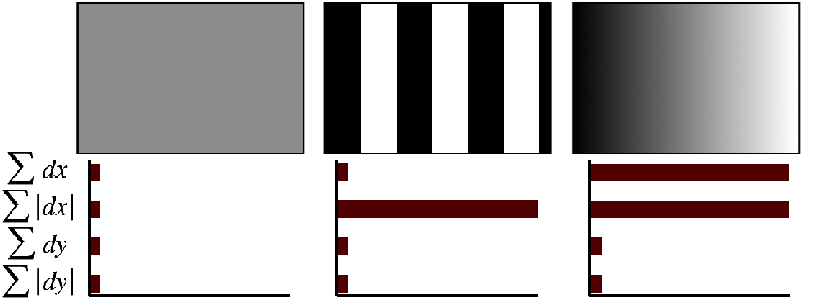
\includegraphics[width=\imsizeS]{histogramas-surf}
\end{center}
\end{minipage}
\hfill
\caption[Calculo del descriptor SURF]
{. Imagen original : \cite{bay2008speeded}.}
\label{fig:haar-wavelet}
\end{figure}


\end{subsection}

\end{subsection}

\begin{subsection}
{Oriented FAST and Rotated BRIEF (ORB)}

ORB es un detector y descriptor \cite{RubleeRKB11} de caracteristicas basado en el detector FAST \cite{Rosten06machinelearning} y el descriptor BRIEF \cite{Calonder12}. Si bien BRIEF es robusto ante cambios de iluminacion y presencia de ruido, es muy sensible a rotaciones in-plane. Teniendo en cuenta este problema, ORB extiende FAST para detectar la orientacion de las caracteristicas (tipo corner) y aplica mejoras sobre BRIEF dirigidas a aprovechar la informacion de orientacion.

\begin{subsection}
{Oriented FAST (oFAST)}

La deteccion de caracteristicas oFAST se compone de 4 etapas :
\begin{enumerate}

\item Deteccion de caracteristicas FAST. Se utiliza un umbral t de intensidad apropiado entre el pixel del centro y los pixeles del anillo circular. En oFAST se utiliza FAST-9 (radio del anillo de 9 pixeles) porque se comprobo que ofrece buenos resultados.

\item FAST no produce una medida de la bondad de los corners y responde positivamente ante la presencia de bordes, por lo que en oFAST se realiza un filtrado con el fin de detectar las mejores caracteristicas. Para obtener los mejores N corners, se aplica una medida de bondad de los corners dada por Harris REFERENCIAR[], se ordena las caractertisticas en funcion de esa medida y se seleccionan las N mejores. Se establece un umbral sufiecientemente bajo para la bondad de los corners, con el fin de obtener al menos N caracteristicas.

\item FAST no produce caracteristicas multi-escala. Para solventar este problema, se construye una piramide de escalas de la imagen (similar a SIFT y SURF), se calcula FAST (filtrado por Harris) en cada nivel y se aplica interpolacion obtener unos mejores resultados. 

\item Estimacion de la orientacion. Para calcular la orientacion se utiliza la medida intensity centroid REFERENCIAR[PAPER] dentro del patch (area rectangular) alrededor del keypoint. Se puede construir un vector O->C desde el centro del corner O hacia el intensity centroid C, y calcular la orientacion del patch como 
\begin{equation}
tita = atan(Cy, Cx)
\end{equation}

\end{enumerate}

\end{subsection}

\begin{subsection}
{Rotated BRIEF (rBRIEF) }

\begin{subsection}
{Binary Robust Independent Elementary Features (BRIEF) }
El descriptor BRIEF REFERENCIA es una cadena de bits (bit string) que describe un patch (centrado en el keypoint) de la imagen. Esta formado por un conjunto de tests binarios aplicados sobre los pixeles. Dado un patch p de la imagen suavizada (mayor robustez frente al ruido), un test binario t se define como : 

\begin{equation}
t(p; x, y) := { 1 : p(x) < p(y), 0 : p(x) >= p(y) }
\end{equation}

donde p(x) es el valor de intensidad de p en la posicion x.
El descriptor se define como un vector de n tests binarios :
fn(p) := sum 1<=i<=n 2**i-1 t (p; xi, yi) 

Hay varios enfoques para la seleccion del conjunto de posiciones a testear. En la version estandar de BRIEF, se utiliza una distribucion Gaussiana alrededor del centro del patch debido a que se comprobo que da los mejores resultados.

\end{subsection}

\begin{subsection}
{Mejoras aplicadas en rBRIEF}

BRIEF posee 2 caracteristicas importantes para un descriptor :
\begin{itemize}

\item Descriptores con elevada varianza y una media cercana a 0.5, lo que permite diferenciar descriptores mas facilmente, dado que distintas caracteristicas responden de forma diferente.

\item Tests poco correlacionados, para que cada uno de ellos aporte informacion distinta y disminuya la redundancia.

\end{itemize}

Estas cualidades se ven disminuidas al agregar la informacion de orientacion. Para solventar este problema, se sigue un enfoque de aprendizaje, por medio del cual se determinan un conjunto de pares de pixeles para ser comparados en cada test. \\
Para comenzar se obtienen los patches centrados en cada keypoint oFAST extraidos a partir de un conjunto de imagenes de entrenamiento. Cada test es un par de sub-ventanas 5x5 pixeles de un patch de 31x31. Da todos los posibles tests, se eliminan aquellos que sobrelapan, finizalizando con un total de M = 205590 posibles tests.
El algorimo se describe como : 

\begin{enumerate}

\item Obtener los resultados del conjunto de tests sobre cada uno de los patches de entranamiento.

\item Ordenar los tests por su distancia a una media de 0.5 formando el vector T. Una media cercana a 0.5 indica alta varianza, mientras que medias alrededor de 0 o 1, indican una varianza menor y una menor capacidad de diferenciacion.

\item Realizar una busqueda greedy de tests poco correlacionados. Se compone de los siguentes pasos : 
\begin{enumerate} {label=(\alph*)}
\item Poner el primer test en el vector resultado R.

\item Escoger el siguiente test de T y compararlo contra todo los tests de R. Si la correlacion absoluta es mayor que un cierto umbral, se descarta; en otro caso se añade a R.

\item Se repite el paso anterior hasta que se dispongan de n = 256 tests. Si no se alcanza esta cantidad, se aumenta el umbral de la correlacion y se repite el paso desde b).

\end{enumerate}
\end{enumerate}

En la figura \ref{fig:correlacion-orb} se muestran los tests binarios aplicando el algoritmo de aprendizaje de tests poco correlacionados frente a la solucion sin aprendizaje.

\begin{figure}[ht]
\centering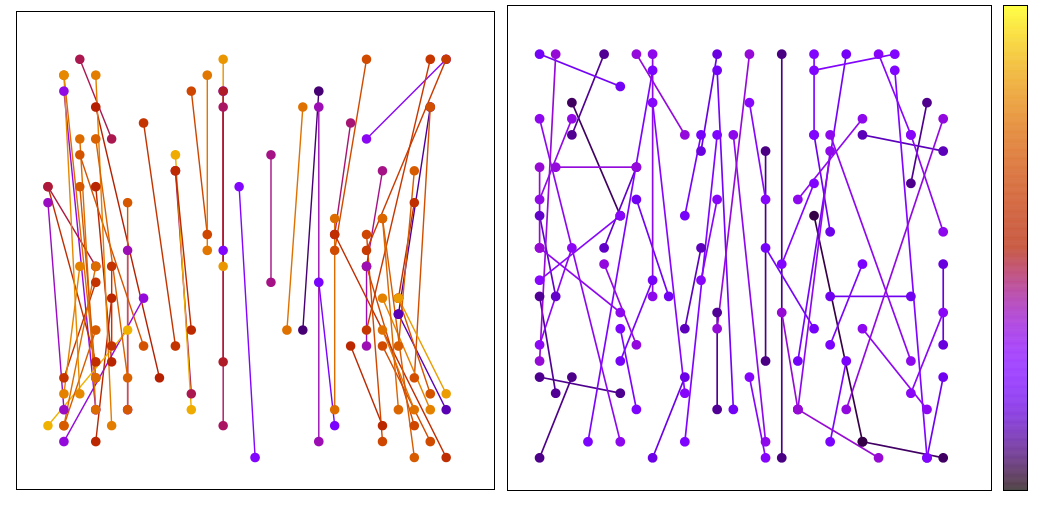
\includegraphics[width=\imsize]
{correlacion-orb}
\caption[Comparacion tests binarios con y sin aprendizaje ORB.]
{ Izquerda : conjunto de tests binarios obtenidos sin aprendizaje (utilizando orientacion con el enfoque de BRIEF). Derecha : conjunto de tests binarios obtenidos por medio del algoritmo de aprendizaje. 	El color violeta indica poco correlacion, mientras que el color naranja representa alta correlacion. Se puede observar que los tests por medio de aprendizaje tienen una mejor distribucion y estan menos correlacionados. Imagen original : \cite{RubleeRKB11}.}
\label{fig:correlacion-orb}
\end{figure}

Para la construccion de cada descriptor, se utiliza la orientacion obtenida en la fase de deteccion como sigue :
\begin{enumerate}

\item Se construye la matriz S de 2xn con las coordenadas de los pares de puntos de los tests, obtenidas a partir del algoritmo de apendizaje.
S = ( x1, ... , xn ; y1, ..., yn )

\item Usando la orientacion del patch teta, se construye la correspondiente matriz de rotacion Rteta y se obtiene la version rotada Steta de S. 

Steta = Rteta S
\item Por ultimo, se utiliza el operador de BRIEF fn(p) sobre los tests rotados obteniendo el operador de rBRIEF. gn(p, teta) := fn(p)|(xi, yi) pertenece Steta.

\end{subsection}

En la implementacion, el algoritmo de aprendizaje se lleva a cabo en un proceso offline. Ademas, se discretizan los angulos en incrementos de 2pi/30 (12 grados) y se construye una lookup table de patrones punto-angulo precalculados.

\end{subsection}

\chapter{Mapa 3D consistente en sistema prototipo}

\section{Filtrado de inconsistencias}
\label{sec:filtrado-estadistico-de-inconsistencias}

En el apartado \ref{sec:consideraciones-kinect}, se explica que el sensor Kinect no esta exento de error y que existen varias restricciones que pueden interferir en las mediciones de profundidad. Aplicando correctamente la técnica de medición digital presentada en la sección \ref{sec:metodologia-medicion-digital}, se disminuye la cantidad de datos incorrectos, pero no hay seguridad de eliminarlos completamente. Por otro lado, al finalizar un ensayo hidráulico, suele permanecer agua acumulada sobre la estructura del dique (con dificultad de drenar sin alterar la condición final del modelo) que puede generar mediciones espurias. \\ 
Con la motivación anterior, se decide aplicar una técnica de análisis estadístico presentada en \cite{Rusu08towards3d}, que busca eliminar mediciones incorrectas. Este enfoque se basa en el cómputo de la distribución de la distancias entre los puntos 3D. Para cada punto, el procedimiento calcula la media $\mu$ y la desviación estándar $\sigma$ de las distancias a sus \textsl{k} vecinos más cercanos. Asumiendo que la distribución resultante es normal $\mathcal{N}(\mu, \sigma^{2})$, todos los puntos que caen fuera del intervalo $\mu \pm \alpha \cdot \sigma$ pueden ser considerados \textit{outliers} y removidos del conjunto de datos. La figura \ref{fig:statistical-removal} muestra el efecto de la eliminación de \textit{outliers} sobre una nube de puntos 3D afectada por el ruido. \\ 
El valor de $\alpha$ depende del tamaño de la vecindad \textsl{k} analizada. En el presente trabajo, se utilizaron los valores $k=20, \alpha=2.5$, dando resultados satisfactorios, considerando aproximadamente 1\% de los puntos como \textit{outliers}.

\begin{figure}[ht]
\centering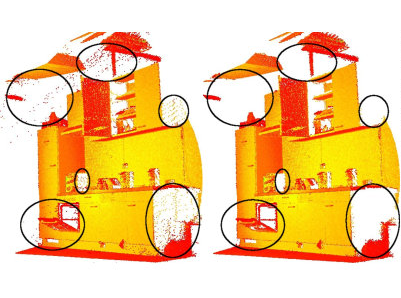
\includegraphics[width=\imsize]
{statistical-removal}
\caption[Eliminación de datos espurios con técnica estadística]
{Efectos del análisis estadístico y eliminación de outliers. Izquierda: la nube de puntos original. Derecha: resultado después de aplicar la técnica estadística \cite{Rusu08towards3d}.}
\label{fig:statistical-removal}
\end{figure}

\section{Mapa 3D en prototipo}
\label{sec:conversion-mapa3D-prototipo}

En ingeniería civil, para realizar estudios de variables sedimentológicas, los datos relevados sobre el modelo son referenciados con el sistema prototipo, es decir, se realiza una conversión a la escala natural de la obra y se define un sistema de coordenadas apropiado. Siguiendo estos lineamientos, se deriva un mapa 3D de la condición de erosión en sistema prototipo, a partir del mapa 3D obtenido en la etapa de registración.\\
En las figuras \ref{fig:sistema-modelo} y \ref{fig:sistema-prototipo} se ilustra una superficie observada desde diferentes sistemas de coordenadas. El sistema modelo (figura \ref{fig:sistema-modelo}) tiene su origen en la cámara Kinect (específicamente en la posición del sensor al iniciar la registración). Para poder realizar la conversión, se requiere asociar una cota (de altitud) en el sistema modelo a una cota en el sistema prototipo (figura \ref{fig:sistema-prototipo}), que defina consistentemente el nuevo sistema de coordenadas. \\ 
Además, se debe aplicar un re-escalado apropiado sobre la escena, debido a la reducción de escala propia de la modelización en laboratorio.\\
Para cada punto 3D $(x_{m}, y_{m}, z_{m})$ en el sistema modelo, la conversión a sistema prototipo $(x_{p}, y_{p}, z_{p})$ esta dada por:
\begin{equation}
x_{p} =   s \cdot x_{m}
\end{equation}
\begin{equation}
y_{p} = - s \cdot y_{m}
\end{equation}
\begin{equation}
z_{p} = - s \cdot (z_{p} - c_{m}) + c_{p}
\end{equation}
donde $c_{m}, c_{p}$ son las cotas de referencia para los sistema de coordenadas modelo y prototipo respectivamente, y \textsl{s} es la escala. \\

\begin{figure}[ht]
\centering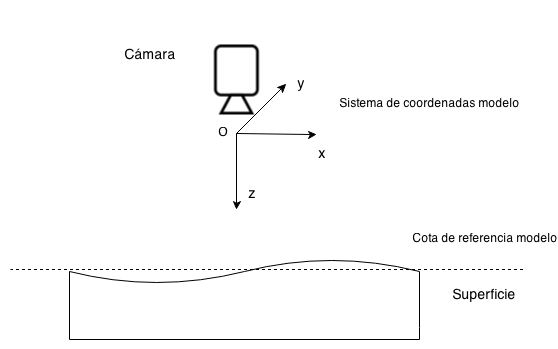
\includegraphics[width=\imsize]
{sistema-coordenadas-modelo}
\caption[Sistema de coordenadas modelo]
{Superficie desde sistema de coordenadas modelo.}
\label{fig:sistema-modelo}
\end{figure}

\begin{figure}[ht]
\centering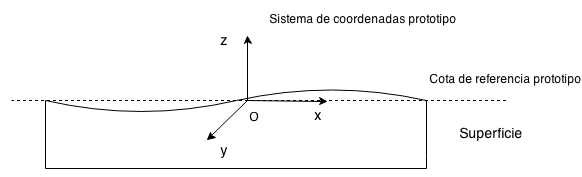
\includegraphics[width=\imsize]
{sistema-coordenadas-prototipo}
\caption[Sistema de coordenadas prototipo]
{Superficie desde sistema de coordenadas prototipo.}
\label{fig:sistema-prototipo}
\end{figure}

En el presente trabajo, la relación de escalas de longitudes modelo prototipo es $s=65$ (propiedad fijada en el modelo físico). La selección de las cotas de referencia varía dependiendo del área de interés en cada ensayo, utilizando siempre que fuera posible, cotas conocidas sobre la estructura del dique, provistas por estudios de topografía.


\chapter{Aplicaciones}

\section{Librerías utilizadas}

Este proyecto ha sido implementado en el lenguaje de programación C++\cite{cplusplus} haciendo extenso uso de librerías \textit{open source}. En primer lugar, se presentan las librerías utilizadas, y de forma seguida, se describe brevemente cómo se aplicaron en este trabajo.

\begin{itemize}

\item OpenNI. (Open Natural Interaction) OpenNI es un conjunto de API’s escritas en C/C++, \textit{open source}, distribuidas bajo la licencia LGPL. Las API's (\textit{Application Programming Interface}) de OpenNI incluyen interfaces de acceso a las cámaras RGB, de rango, micrófonos, así como componentes de más alto nivel como detección de gestos, \textit{skeleton tracking}, etc.
Son soportadas por la organización sin ánimo de lucro, OpenNI, liderada por la industria y centrada en la mejora de los dispositivos de interacción de forma natural. Uno de sus socios principales es PrimeSense, empresa responsable de la tecnología que utiliza el sensor Kinect. 

\item OpenCV. (Open Source Computer Vision Library) Librería escrita en C/C++, multiplataforma y \textit{open source}, distribuida bajo la licencia BSD. La librería OpenCV incluye algoritmos de procesamiento de imágenes y de visión por computadora como emparejamiento de características, visión estéreo, detección de objetos, etc.

\item PCL. (Point Cloud Library) Librería escrita en C++, multiplataforma y \textit{open source}, distribuida bajo la licencia BSD. La librería PCL incluye algoritmos para el procesamiento de nubes de puntos n-dimensionales y geometría 3D, así como métodos específicos para realizar filtrado, segmentación, detección de características, reconstrucción 3D, etc.

\item Eigen. Librería escrita en C++, open source, distribuida bajo la licencia LGPL. La librería incluye métodos de álgebra lineal; como operaciones sobre matrices y vectores, métodos numéricos de resolución de sistemas lineales, etc.

\item FLANN. (Fast Library for Approximate Nearest Neighbors) Librería escrita en C++, multiplataforma y \textit{open source}, distribuida bajo la licencia BSD. La librería FLANN incluye algoritmos para realizar búsquedas de los vecinos más cercanos en espacios de elevada dimensión.

\item Boost. Conjunto de librerías escritas en C++, multiplataforma y \textit{open source}, distribuidas bajo la licencia Boost Software License. Las librerías Boost incluyen métodos para algebra lineal, \textit{multithreading}, \textit{smart pointers}, procesamiento de imágenes, test unitarios, etc.

\item VTK. (Visualization Toolkit) Librería escrita en C++, multiplataforma y \textit{open source}, distribuida bajo la licencia BSD. La librería incluye una amplia variedad de algoritmos para visualización de texturas, volúmenes, etc.

\end{itemize}

Conceptualmente, el proyecto puede dividirse en varios bloques de software, que se describen a continuación :
\begin{itemize}

\item Captura y almacenamiento de datos: se utiliza el formato PCD (\textit{Point Cloud Data}), propio de PCL, para el almacenamiento de nubes de puntos. Para capturar los datos provistos por la Kinect, se utiliza un API provista por PCL, que por debajo interactúa con el driver OpenNI para acceder al dispositivo. Se aprovecha el modo de captura sincronizada de frames RGB y de profundidad (implementado en OpenNI) para integrar la información en nubes de puntos RGB-D.

\item Procesamiento de imágenes 2D: OpenCV provee algoritmos para la detección de características 2D, entre ellos destacan las implementaciones de ORB y SURF, y procedimientos para determinar correspondencias con descriptores binarios y reales.

\item Procesamiento de nubes de puntos 3D: PCL contribuye en múltiples etapas en el proceso de registración : provee la aproximación de la pose utilizando SVD y soporta varias versiones de ICP para el refinamiento de la transformación rígida. Contiene una implementación genérica de RANSAC, que puede ser instanciada con el modelo de transformación rígida para eliminar outliers 3D. En el terreno de \textit{GraphSLAM}, brinda una estructura para construir el grafo de poses e implementa un algoritmo para optimización global basado en el enfoque de Lu y Milios. Por último, cabe destacar que PCL cuenta con varios métodos de filtrado de puntos, entre ellos la técnica de filtrado estadístico presentada en la sección \ref{sec:filtrado-estadistico-de-inconsistencias}.

\item Visualización de datos: se utiliza el \textit{framework} de visualización de nubes de puntos 3D provisto por PCL, construido encima de la librería VTK.

\item Librerías auxiliares de propósito específico: PCL y OpenCV implementan sus algoritmos apoyados en otras librerías open source que llevan a cabo tareas más específicas. Para manejar vectores y transformaciones (representadas por matrices) PCL utiliza Eigen, que soporta operaciones de álgebra lineal. Boost se encarga del manejo automático de la memoria en PCL y contiene estructuras para construir el grafo de poses. Tanto OpenCV como PCL se apoyan en FLANN para realizar búsquedas de vecinos más cercanos, el primero en espacios de grandes dimensiones, mientras que el último principalmente en 3D.

\end{itemize}

\section{Aplicaciones}

Este proyecto se ha implementado y probado sobre el sistema operativo Ubuntu \cite{ubuntu} y requiere de las librerías \textit{open source} citadas en la sección anterior. El sistema se divide en dos componentes, la aplicación \textit{ModelMapper} que genera un mapa 3D (en sistema modelo) a partir de la condición de erosión del modelo físico y la aplicación \textit{RealWorldConverter} que filtra inconsistencias y retorna un mapa 3D convertido a sistema prototipo. Para simplificar la implementación, se utiliza una interfaz de líneas de comandos \cite{wiki-linea-de-comandos}, estándar en sistemas GNU/Linux \cite{wiki-gnu-linux}.

\subsection{\textit{ModelMapper}}
\label{sec:model-mapper}
La finalidad de esta aplicación es generar un mapa 3D de una zona de interés del físico sobre el que se trabaja. Toma nubes de puntos RGB-D como entrada y devuelve las nubes de puntos alineadas en el sistema de coordenadas modelo (apartado \ref{sec:conversion-mapa3D-prototipo}) utilizando la técnica de registración presentada en \ref{sec:descripcion-general-registracion}. \\
Al finalizar la registración, las nubes de puntos alineadas se almacenan en un directorio llamado \textit{registration}, creado (automáticamente) dentro de un directorio \textit{base} especificado por el usuario. La ruta del directorio \textit{base} se ingresa a través de la opción --output-dir (requerimiento obligatorio). \\
La opción --backup habilitar el guardado de las nubes de puntos de entrada (a medida que se van procesando) en un directorio llamado \textit{backup}, creado (automáticamente) dentro del directorio \textit{base}. Deshabilitada por default.\\

Se plantearon dos métodos para ingresar las nubes de puntos, que se pueden seleccionar utilizando la opción --mode.
Los valores aceptados son \textsl{camera} (modo cámara) y \textsl{files} (modo archivos). Por default se trabaja en modo cámara.
\begin{itemize}

\item Modo cámara: los frames RGB-D son capturados directamente desde el sensor Kinect y registrados inmediatamente. En la figura REFERENCIAR[FIGURA], se muestra la pantalla observada en este modo. A la izquierda, se visualiza la última nube de puntos capturada. A la derecha, se observa el estado parcial de la registración. Se requiere presionar la tecla \textit{espacio} para ingresar un nuevo frame. Presionando la tecla \textit{p} se finaliza la registración.

AGREGAR CAPTURA DE PANTALLA

\item Modo archivos: los frames RGB-D son obtenidos desde el sistema de archivos. Este modo está pensado para correr el proceso de registración con frames capturados con el modo cámara (con la opción --backup habilitada) y probar diferentes parametros para el algoritmo de registracion (los cuales se explicaran en los párrafos siguientes). Se requiere ingresar la opción --input-dir seguida del directorio \textit{base} que contiene la carpeta \textit{backup}. Este modo es completamente automático, es decir, que no requiere interacción alguna por parte del usuario (nota: no se muestra el visualizador con las nubes de puntos).

\end{itemize}

A continuación, se lista una serie de parametros del algoritmo de registracion que pueden ser modificados desde la interfaz de líneas de comandos:

\begin{itemize}

\item Option --features: tipo de algoritmo para extraer características visuales. Posibles valores: \textsl{surf, orb}. Default : \textsl{orb}. Detalles en el apartado \ref{sec:features}.

\item Opción --min-num-inliers: mínima cantidad de correspondencias correctas para considerar que la odometría fue medida exitosamente. Default: 45. Detalles en el apartado frontend de \textit{GraphSLAM} \ref{sec:slam-frontend}.	

\item Opción --min-num-extra-inliers: mínima cantidad de correspondencias correctas para la detección de bucles en un mapa. Default: 25. Detalles en el apartado frontend de \textit{GraphSLAM} \ref{sec:slam-frontend}.

\item Opción --extra-edges: Máxima cantidad de aristas con las que se puede extender el grafo de poses en la etapa de detección de bucles. Default: 2. Detalles en el apartado frontend de \textit{GraphSLAM} \ref{sec:slam-frontend}.

\end{itemize}

Se destaca que esta aplicación explícitamente almacena el mapa 3D dividido en varios archivos PCD. 

\,section{\textit{RealWorldConverter}}
 
Esta aplicación cumple dos tareas, eliminar posibles inconsistencias del mapa 3D generado con ModelMapper utilizando la técnica de filtrado estadístico (explicada en la sección \ref{sec:filtrado-estadistico-de-inconsistencias}) y generar un mapa 3D en sistema prototipo (presentado en la sección \ref{sec:conversion-mapa3D-prototipo}) para que pueda ser utilizado en estudios de la erosión.

ModelMapper almacena el mapa 3D dividido en diferentes archivos debido a que RealWorldConverter brinda la posibilidad de seleccionar un subconjunto del total de nubes de puntos, con la finalidad de crear un mapa más liviano o de una zona específica. 

Los parámetros obligatorios a ingresar en esta aplicación son:

\begin{itemize}
\item Opción --input $ cloud_{1}, ..., cloud_{n} $: lista de nubes de puntos de entrada.

\item Opción --output cloud\_final.pcd: path para almacenar el mapa 3D filtrado en sistema prototipo.

\item Opción --scale s: factor de escala.

\item Opción --real\_base r: cota de referencia en prototipo.

\end{itemize}

Para ingresar la cota de referencia en modelo hay dos posibilidades: 
\begin{itemize}

\item Ingresar la opción --model\_base m, donde m es valor de la cota.

\item Visualizar el mapa 3D en sistema modelo y seleccionar un punto 3D (con la combinación shift + click derecho) para utilizar su altitud como cota de referencia en modelo.

\end{itemize}

% Hay dos parametros opcionales para configurar el algoritmo de filtrado estadístico:
% AGREGAR PARAMETROS




\chapter{Medición de erosión en un modelo físico de laboratorio}

\section{Descripción del modelo}

Los ensayos llevados a cabo en este trabajo se realizaron en un modelo físico ubicado en el Laboratorio de Hidráulica de la Facultad de Ciencias Exactas, Físicas y Naturales (UNC). El modelo es una representación del Dique Los Molinos a escala reducida de longitudes 1:65. Este Dique se encuentra ubicado en la provincia Jujuy, sobre el río Grande, aguas debajo de la confluencia con el río Reyes. \\
El modelo físico hidráulico está representado con fondo fijo en las márgenes y fondo móvil en el lecho del río. Se representaron las obras de regulación, con todos sus componentes y elementos auxiliares de relevancia hidrosedimentológica. Cuenta con un tramo del curso fluvial con un desarrollo total de aproximadamente 1520 m (1000 m aguas arriba y 520 m aguas abajo del dique), y un ancho efectivo variable entre los 250 m a 700 m en prototipo. Estas características permiten analizar adecuadamente el comportamiento hidrosedimentológico del flujo en cercanías de las obras, el funcionamiento de las operaciones de maniobra y la erosión en el tramo de río aguas abajo del dique. Como se observa en la figura \ref{fig:modelo-fisico-dique-los-molinos}, el dique está constituido por un terraplén de materiales sueltos y dos vertederos, un tramo a nivel fijo (dique fijo), y otro regulado por 4 compuertas, conocido como dique móvil. Sobre margen derecha, se encuentra el canal moderador.

\begin{figure}[ht]
\centering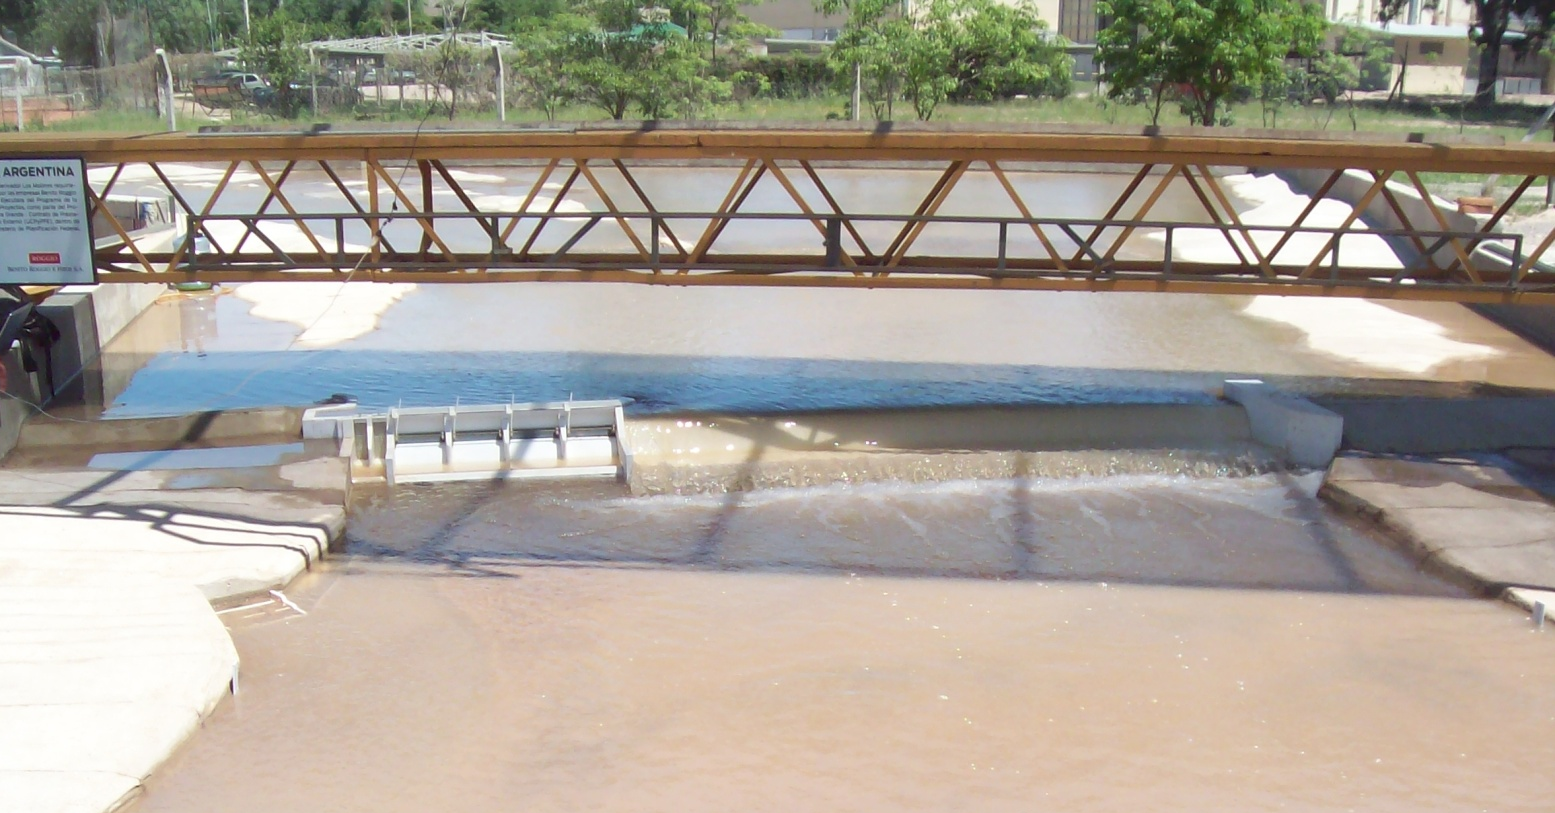
\includegraphics[width=\imsize]
{modelo-fisico-dique-los-molinos}
\caption[Modelo físico dique Los Molinos]{Modelo físico dique Los Molinos, Laboratorio de Hidráulica, FCEFyN de la UNC.}
\label{fig:modelo-fisico-dique-los-molinos}
\end{figure}

\begin{figure}[ht]

\centering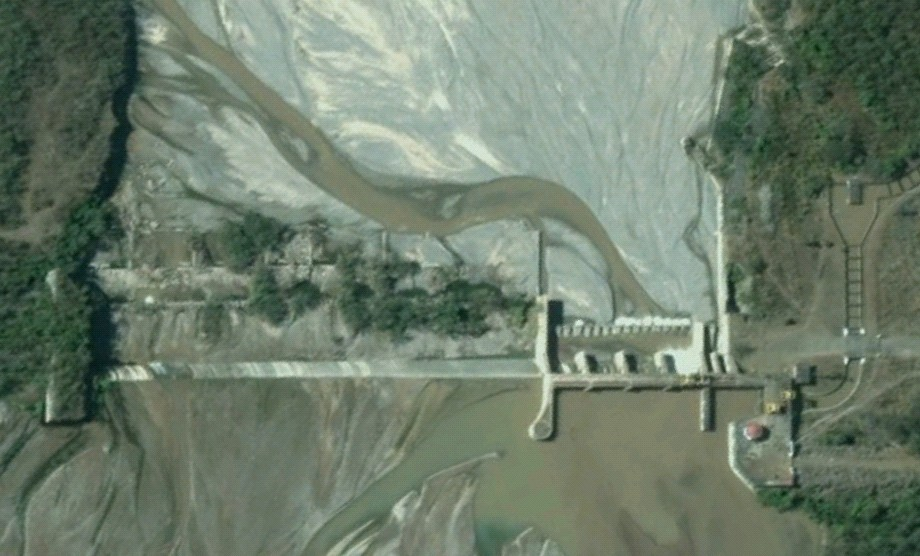
\includegraphics[width=\imsize]
{dique-los-molinos}
\caption[Dique Los Molinos]{Dique Los Molinos, Jujuy.}
\label{fig:dique-los-molinos}

\end{figure}

Teniendo en cuenta el alcance de este trabajo, los objetivos para el estudio sobre este modelo fueron los siguientes:
\begin{itemize}

\item Analizar y cuantificar las erosiones locales, aguas abajo de las estructuras de descarga a los fines de constatar el funcionamiento de las obras previstas en el proyecto. Esta evaluación se llevará a cabo para escenarios hidrológicos de diseño.

\item Verificar y optimizar las consignas de operación de las estructuras de control, a los fines de regular los procesos hidrosedimentológicos frente a crecientes aguas arriba del dique móvil.

\end{itemize}

Sobre la zona relevante, se ha construido una plataforma móvil que posibilita realizar las mediciones de erosión. Figura \ref{fig:sistema-camara-carro}. Sus componentes principales son:

\begin{itemize}

\item Un puente grúa. Este puede ser trasladado para observar distintas áreas del modelo.

\item Una guía-riel y un carro-soporte para la cámara Kinect. La guía se anexa al puente grúa, lo que permite la traslación de la cámara a lo ancho del modelo.

\end{itemize}

\begin{figure}[ht]
\centering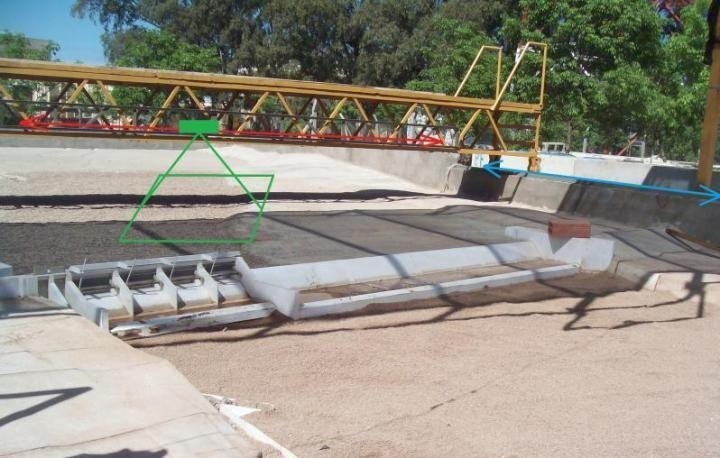
\includegraphics[width=\imsize]
{esquema-camara-puente-grua}
\caption[Puente grúa]{Puente grúa. Las flechas indican la direcciones en la que se puede trasladar la cámara (esquematizada con el recuadro verde). En rojo, traslación utilizando el carro soporte, mientras que la trayectoria en azul, se consigue movilizando el puente grúa.}
\label{fig:esquema-camara-puente-grua}
\end{figure}

\begin{figure}[ht]
\centering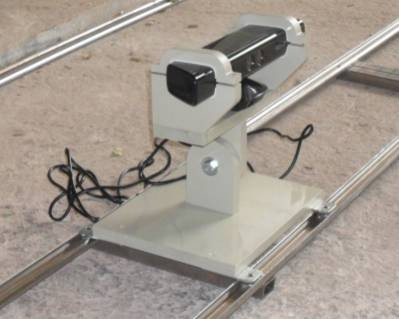
\includegraphics[width=\imsizeS]
{sistema-camara-carro}
\caption[Sistema cámara-soporte]{Soporte construido para trasladar la cámara sobre el modelo.}
\label{fig:sistema-camara-carro}
\end{figure}

%%%%%%%%%%%%%%%%%%%%%%%%%%%%%%%%%%%%%%%%%%%%%%%%%%%%%%%%%%%%%%%%%%%%%%%%%%%%%%%

\section{Etapas de un ensayo hidráulico}
\label{sec:etapas-previas-medicion}

En cada ensayo hidráulico realizado, se cubrieron las etapas enumeradas a continuación:  
\begin{enumerate}

\item Se estableció la condición inicial del modelo, aguas abajo de las estructuras, nivelando el material suelto (arena) hasta la cota del terreno medido con la topografía provista. Figura \ref{fig:condicion-inicial-modelo}. Se utilizó una cota media de 1360 m s.n.m.

\item Encendido del modelo. Se encienden las bombas hidráulicas y comienza a recircular el agua dentro de cisternas y canales de aforos del laboratorio. Se realiza un manejo del sistema de bombeo hasta alcanzar el caudal establecido para cada  ensayo o escenario a simular.

\item Monitoreo de la erosión durante cada ensayo hasta alcanzar la condición de estabilidad. Estas mediciones se llevan a cabo con nivel óptico y mira. Se realizan mediciones de nivel en las zonas de interés durante intervalos temporales regulares, hasta medir valores similares entre estos intervalos.

\item Apagado del modelo. Se apagan las bombas hidráulicas, se cierran las compuertas correspondientes, y se deja drenar el modelo.

\item Medición de erosión. Esta etapa se desarrollará en detalle en las siguientes secciones.

\end{enumerate}

\begin{figure}[ht]
\centering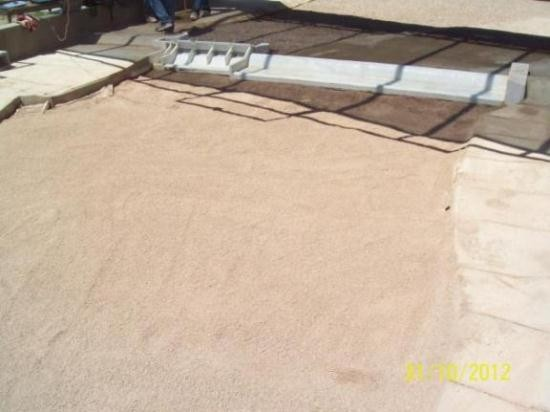
\includegraphics[width=\imsizeS]
{condicion-inicial-modelo}
\caption[Condición inicial del modelo]
{Condición inicial del modelo}
\label{fig:condicion-inicial-modelo}
\end{figure}

%%%%%%%%%%%%%%%%%%%%%%%%%%%%%%%%%%%%%%%%%%%%%%%%%%%%%%%%%%%%%%%%%%%%%%%%%%%%%%%

\section{Metodología de medición con nivel óptico}

La técnica tradicional consiste en el relevamiento manual de puntos sobre perfiles longitudinales y transversales (en la figura \ref{fig:esquema-perfiles}), por lo general cada 10 cm, utilizando para dicha tarea el nivel óptico (en la figura \ref{fig:nivel-optico}) y una mira con una escala graduada al milímetro.  

\begin{figure}[ht]
\centering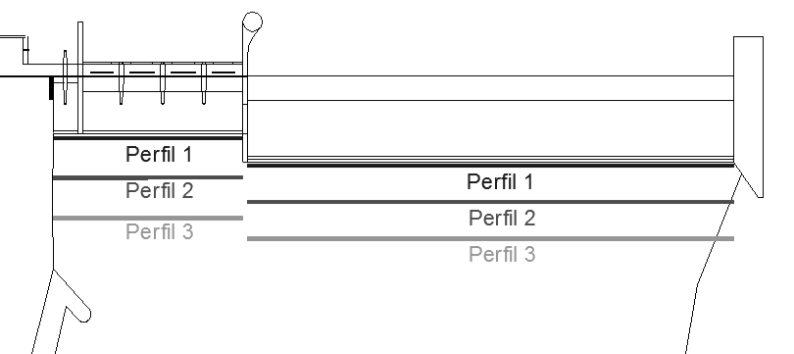
\includegraphics[width=\imsize]
{esquema-perfiles}
\caption[Perfiles transversales]
{Ubicación de perfiles transversales para medir las erosiones finales.}
\label{fig:esquema-perfiles}
\end{figure}

\begin{figure}[ht]
\centering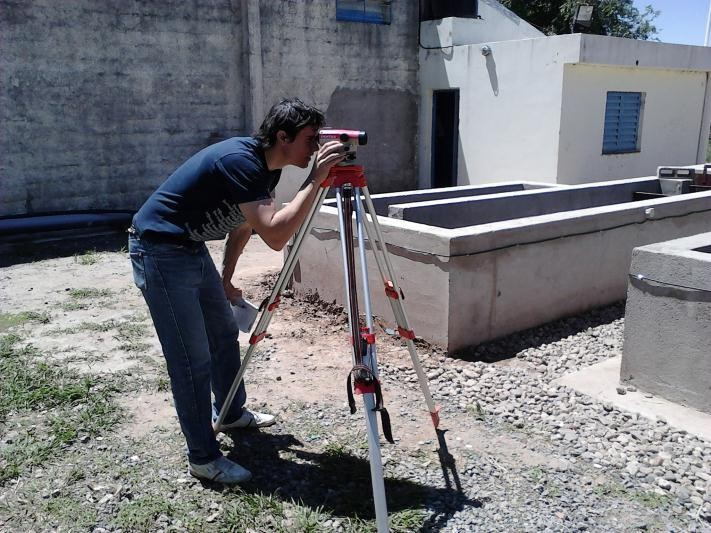
\includegraphics[width=\imsize]
{nivel-optico}
\caption[Nivel óptico]
{Medición con nivel óptico en modelo físico Los Molinos, cortesía de Nicolás Bellino.}
\label{fig:nivel-optico}
\end{figure}

Por último, se realiza la digitalización manual y conversión de modelo a prototipo de los puntos relevados. \\
Cabe destacar que para implementar esta técnica suelen participar 3 personas e invertir aproximadamente 20 minutos por cada metro cuadrado, relevando puntos cada 15 cm.
\section{Metodología de medición con cámara RGB-D}
\label{sec:metodologia-medicion-digital}

En esta sección, se describe la aplicación de la técnica digital de medición de erosión propuesta en este trabajo. \\

Se tuvieron en cuenta un conjunto de consideraciones que forman parte de la técnica de medición y permiten obtener resultados óptimos, las cuales se presentan a continuación:

\begin{itemize}

\item La superficie a relevar debe estar libre de agua. Como se mencionó en el apartado \ref{sec:consideraciones-kinect}, se observó que los objetos con características reflectantes afectan al sensor de profundidad de la Kinect. Figura \ref{fig:modelo-condiciones-agua}.

\item La escena debe estar al resguardo de la luz solar, como se explica en el apartado \ref{sec:consideraciones-kinect}. Debido a que el modelo físico utilizado se encuentra al aire libre, en el exterior del Laboratorio de Hidráulica, fue necesario utilizar un nailon de color negro colocado sobre el puente grúa, como se puede observar en la figura \ref{fig:modelo-lona}. Alternativamente, se consideró realizar las mediciones al atardecer cuando la luz solar es más tenue. Se concluye que utilizando el nailon se obtienen condiciones lumínicas estables, quitando así una restricción para el horario de medición.

\item La guía debe estar horizontalizada. El plano desde el que se captura la escena debe estar a una altitud constante para que la representación de la superficie sea consistente. Esta condición debe ser verificada al iniciar cada ensayo hidráulico.

\item La cámara debe ubicarse en un rango de 0.4 m  a 1.5 m de altura sobre la escena a relevar, para que el error de medición se mantenga dentro del intervalo aceptable (aproximadamente 5 mm), según el análisis del sensor Kinect presentado en el apartado \ref{sec:consideraciones-kinect}.

\end{itemize}

\begin{figure}[ht]
\centering
\begin{minipage}[t]{.45\textwidth}
\begin{center}
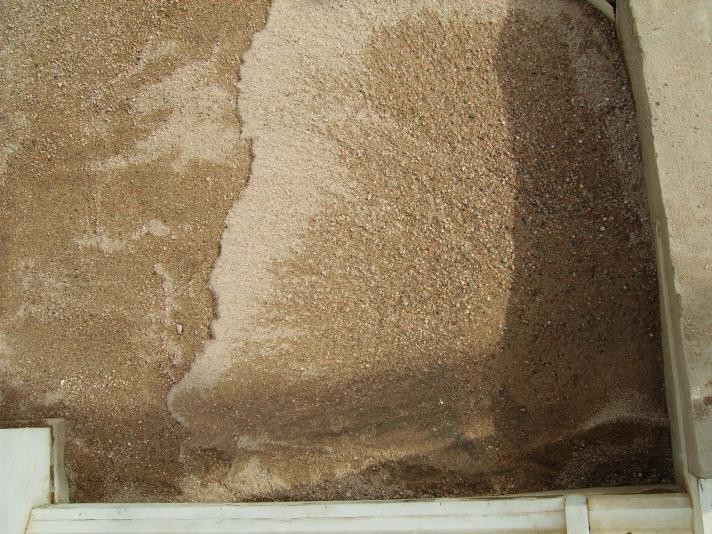
\includegraphics[width=\imsizeS]{modelo-sin-agua} % primera imagen colocada a la izquierda
\end{center}
\end{minipage}
\hfill
\begin{minipage}[t]{.45\textwidth}
\begin{center}
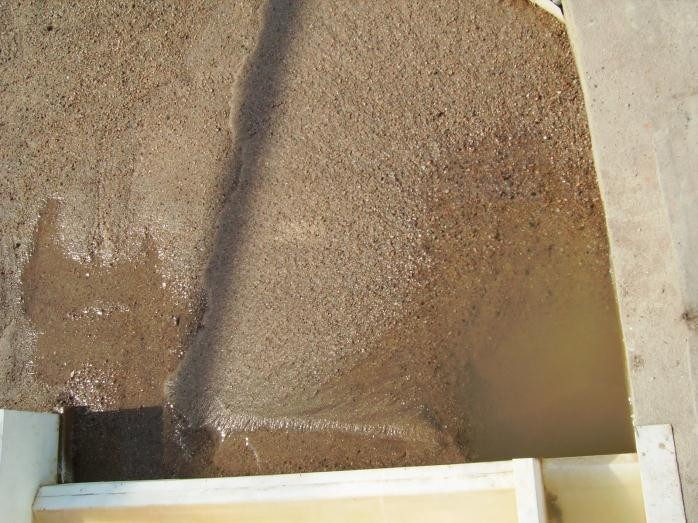
\includegraphics[width=\imsizeS]{modelo-con-agua} % segunda imagen colocada a la derecha
\end{center}
\end{minipage}
\hfill
\caption[Modelo físico con y sin agua sobre la superficie]{Derecha: condición correcta para la medición. Izquierda: se observan espejos de agua que interfieren el sensor infrarrojo de la cámara.}
\label{fig:modelo-condiciones-agua}
\end{figure}

\begin{figure}[ht]
\centering
\begin{minipage}[t]{.45\textwidth}
\begin{center}
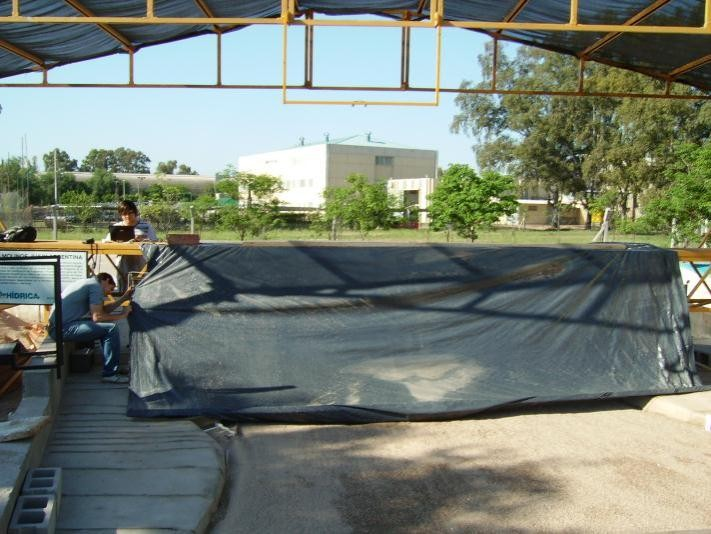
\includegraphics[width=\imsizeS]{modelo-lona1} % primera imagen colocada a la izquierda
\end{center}
\end{minipage}
\hfill
\begin{minipage}[t]{.45\textwidth}
\begin{center}
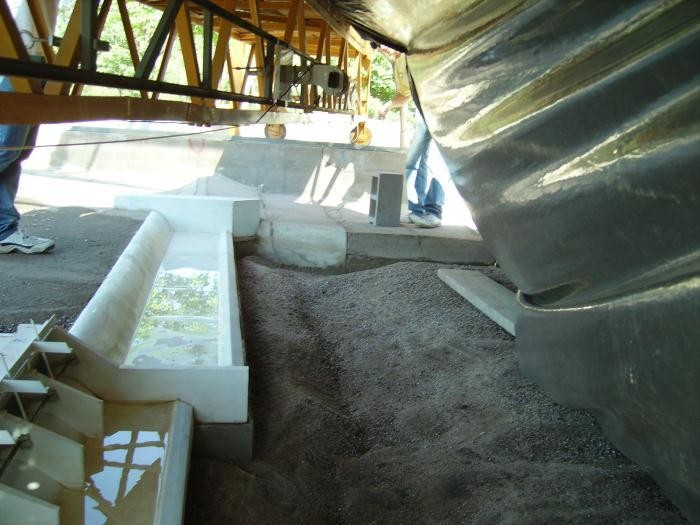
\includegraphics[width=\imsizeS]{modelo-lona2} % segunda imagen colocada a la derecha
\end{center}
\end{minipage}
\hfill
\caption[Nailon utilizado para evitar interferencia de luz solar]{Derecha: Forma de colocar el nailon sobre el puente grúa para cubrir todo el largo del riel. Izquierda: La sombra producida por el nailon permite capturar las imágenes sin interferencia del sol.}
\label{fig:modelo-lona}
\end{figure}

Habiendo verificado las condiciones anteriores, se introduce el carro-soporte en el carril-guía y se inicia la aplicación de registración \textit{ModelMapper} \ref{sec:model-mapper}. \\
 
En la figura \ref{fig:aguas-abajo-desplazamiento-carro}, se observa cómo manipular la plataforma móvil para capturar la escena. Se propone un desplazamiento del carro de aproximadamente 40 cm entre cada captura, para que el área superpuesta entre dos nubes puntos consecutivas esté próxima al 50\%. Si la aplicación no lograr realizar la registración correctamente se corrige la ubicación del sensor a una posición intermedia.

\begin{figure}[ht]
\centering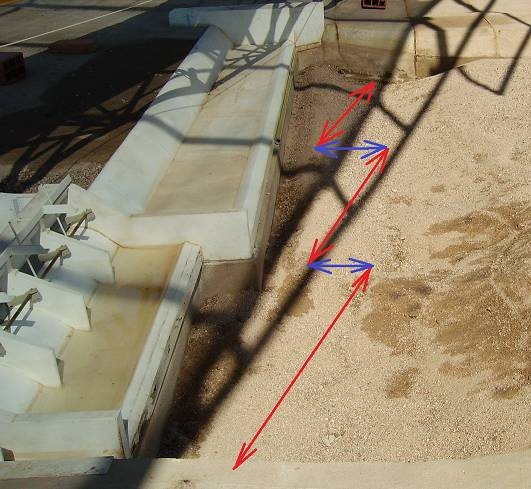
\includegraphics[width=\imsize]
{aguas-abajo-desplazamiento-carro}
\caption[Desplazamiento de la cámara]{Recorrido del puente grúa y del carro-soporte sobre la escena. Las flechas rojas indican desplazamiento de la cámara y las flechas azules representan el movimiento del puente.}
\label{fig:aguas-abajo-desplazamiento-carro}
\end{figure}

En el apartado \ref{sec:conversion-mapa3D-prototipo} se describe que para realizar la conversión a prototipo es necesario un punto fijo con cotas conocidas en los sistemas del modelo y del prototipo. Con este fin, se recomienda que la escena capture las estructuras fijas en el modelo físico con medidas de elevación dada por mediciones topográficas. En caso contrario, se puede medir con nivel óptico un punto visible en la escena y utilizar su cota prototipo como referencia. \\
Utilizando la técnica digital se invierte aproximadamente 1 min para trasladar la cámara y procesar un nuevo frame. Teniendo en cuenta que se requieren 6 frames (aprox.) por $m^{2}$ y posiblemente se descarte algún frame en el proceso, se estiman 10 min para relevar un área de un $m^{2}$. Comparando con la técnica tradicional, se observa que se reduce por la mitad el tiempo invertido para cada ensayo.

%%%%%%%%%%%%%%%%%%%%%%%%%%%%%%%%%%%%%%%%%%%%%%%%%%%%%%%%%%%%%%%%%%%%%%%%%%%%%%%

\section{Ensayos realizados}
En la tabla siguiente se presenta un resumen de los ensayos realizados. Se detallan los caudales asociados así como las estructuras hidráulicas por las que pasa cada uno y su representatividad.\\

\begin{tabular}{ccc}
\hline
Ensayo  & Caudal total $m^{3}/s$ & Motivación \\
\hline
1 & 900 & Caudal Máximo Dique Móvil (DM) y \\
  &     & Canal Moderador (CM) \\
\hline
2 & 3200 & Caudal Máximo Sólo Dique Fijo (DF) \\
\hline
3,7,9 & 4200 & Caudal para Periodo de Retorno T=10000 años \\
\hline
4 & 90 & Caudal de Despegue CM \\
\hline
5 & 225 & Caudal de Despegue DM \\
\hline
10 & 600 & Caudal de Verificación DF, DM y CM
 \\
\hline
13 & 1600 & Caudal de Verificación DF, DM y CM
 \\
\hline
14 & 600 & Caudal de Verificación DM y CM
 \\
\hline
\end{tabular}

\newpage % Salto de página para acomodar las imágenes

\subsection{Medición de erosión máxima}
\label{sec:ensayo-erosion-maxima}

En el ámbito de la Ingeniería Civil, la representación con modelos físicos a escala reducida y la simulación de ensayos hidráulicos fluviales, como los que aquí se presentan, tiene entre sus objetivos principales definir las cotas de erosión máxima. Estas mediciones se realizan con el fin de establecer las profundidades de fundación de los muros de contención de las estructuras hidráulicas que componen el sistema evaluado. \\
Se muestran los mapas de elevación en escala prototipo, generados a partir del relevamiento de fosos de erosión ubicados aguas abajo de las estructuras, para los ensayos 1 y 3. Como punto de referencia se utilizó la parte superior del dique móvil, con cota igual a 1377.77 m s.n.m.\\

\begin{figure}[ht]
\centering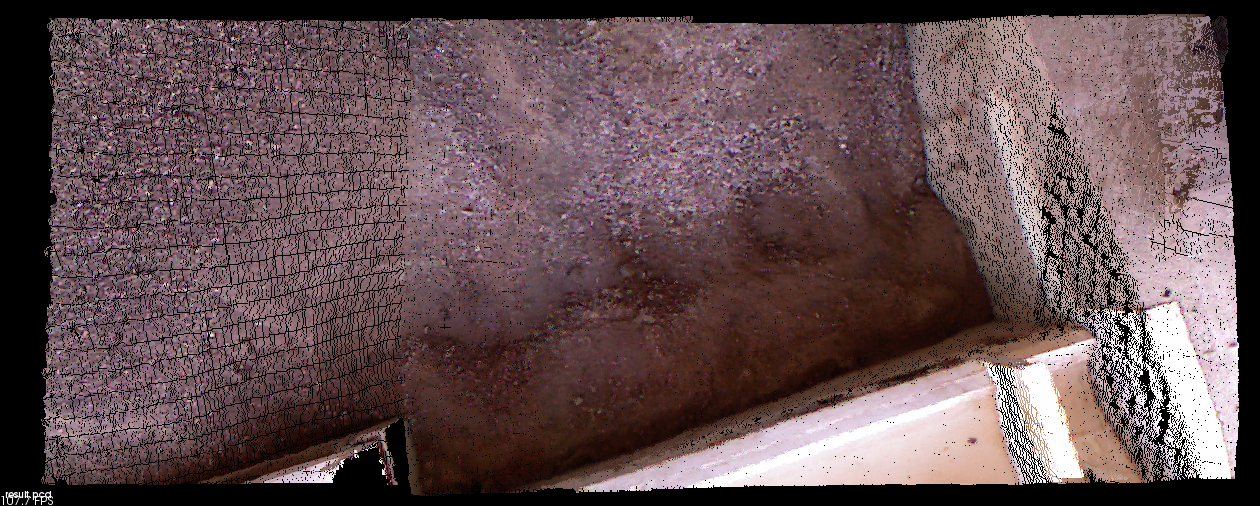
\includegraphics[width=\imsizeL]
{Q900_rgb}
\caption[Imagen RGB Ensayo 1]
{Ensayo 1. Foso de erosión aguas abajo del dique móvil.  Imagen RGB.}
\label{fig:Q900_rgb}
\end{figure}

\begin{figure}[ht]
\centering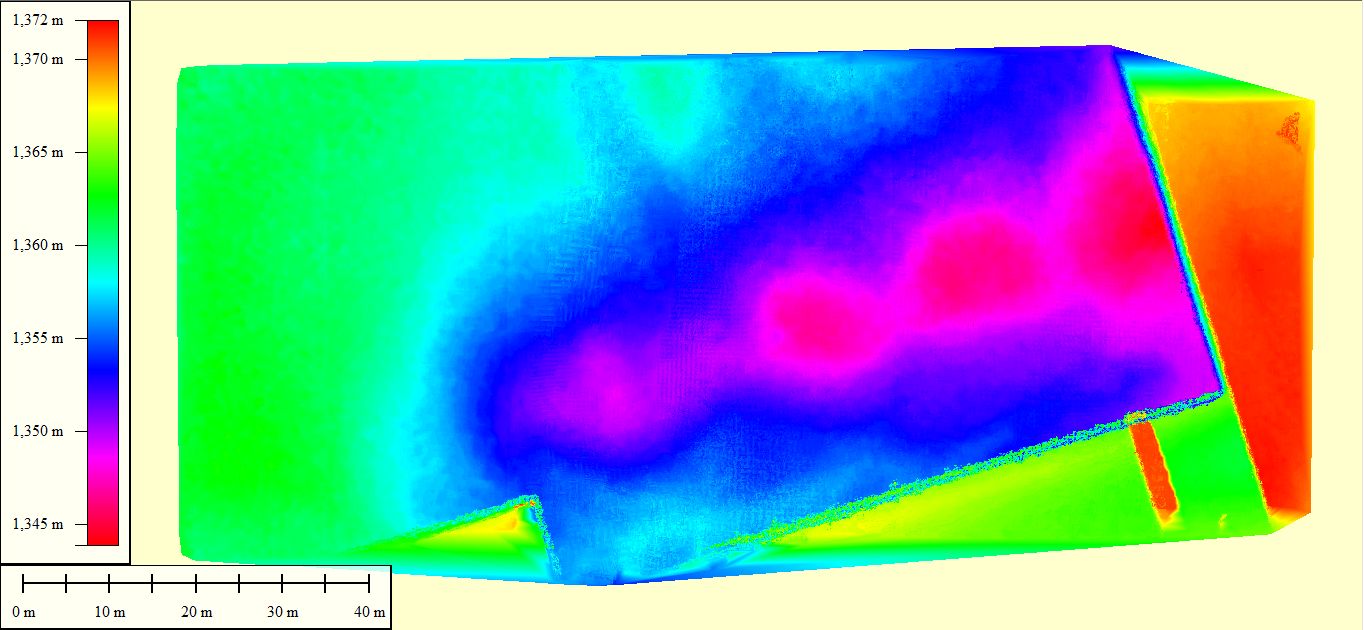
\includegraphics[width=\imsizeL]
{Q900_dem}
\caption[DEM Ensayo 1]
{Ensayo 1. Foso de erosión aguas abajo del dique móvil. Modelo digital de elevaciones.}
\label{fig:Q900_dem}
\end{figure}

\begin{figure}[ht]
\centering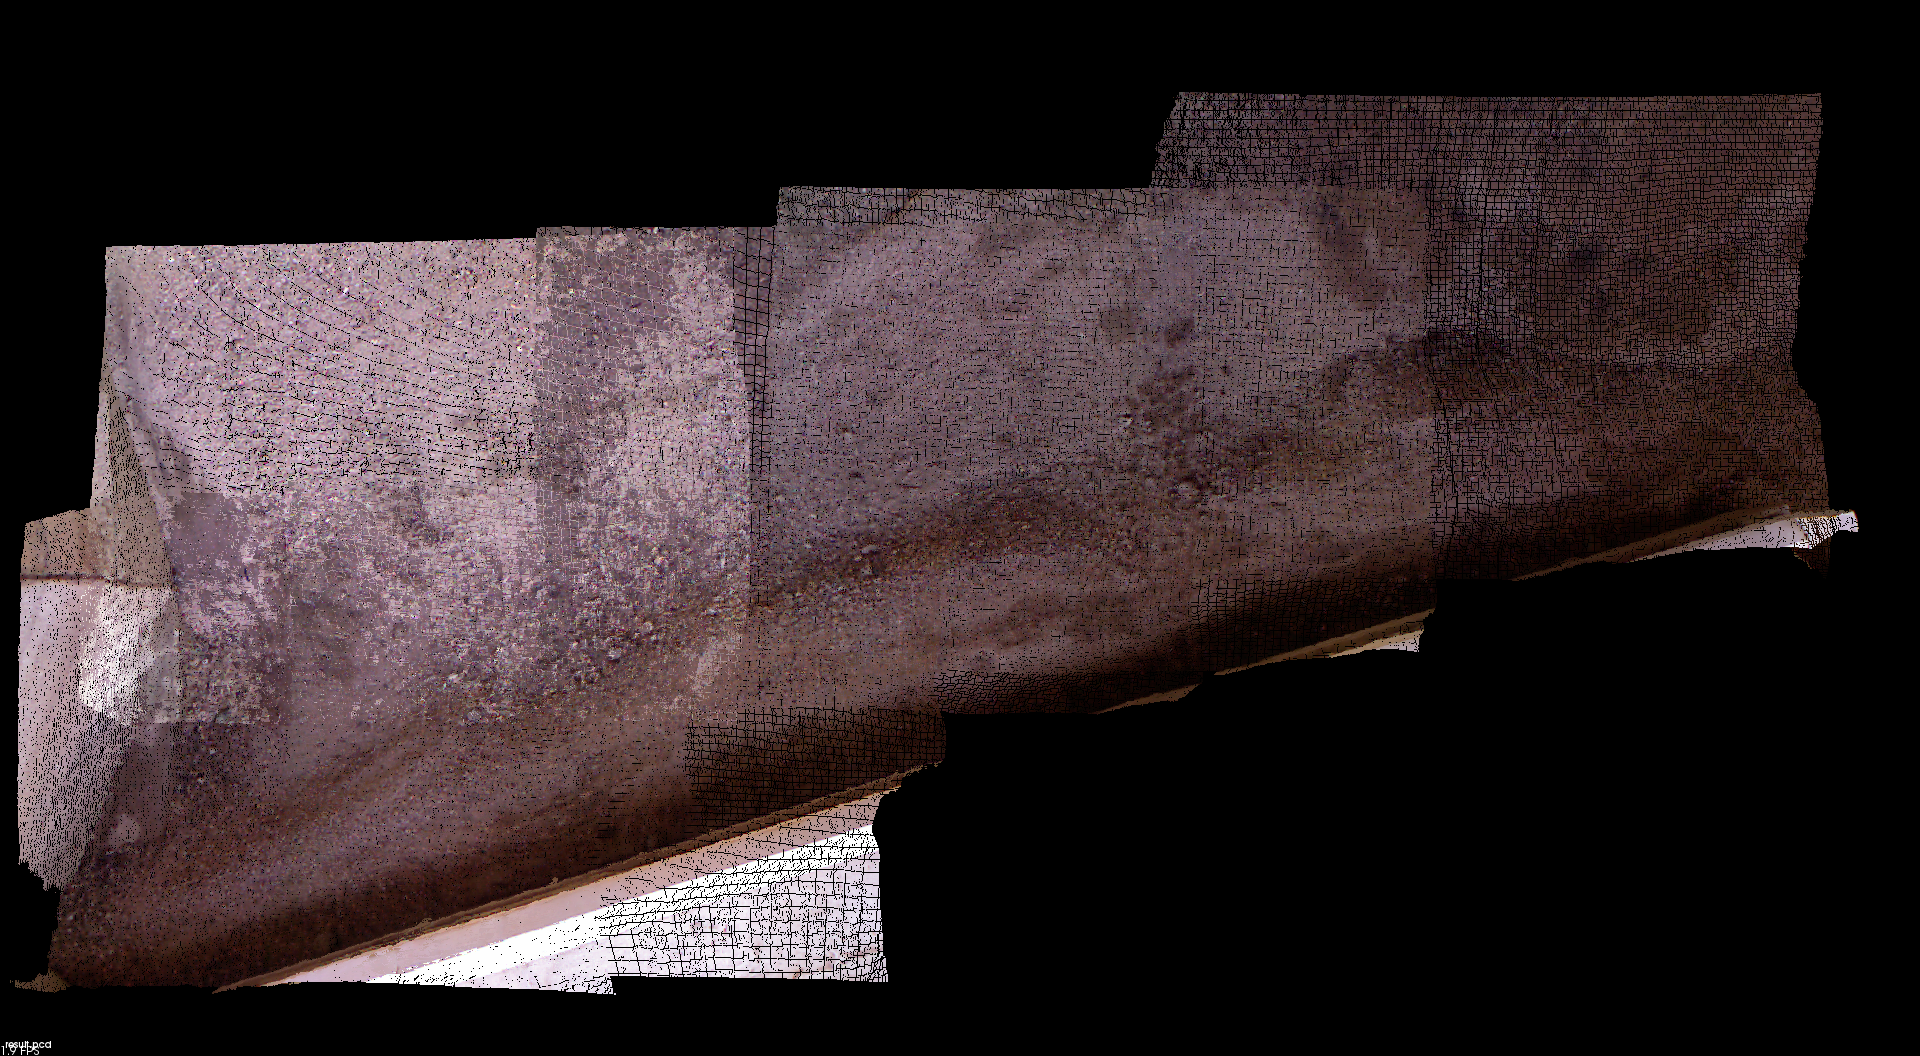
\includegraphics[width=\imsizeL]
{Q4200_rgb}
\caption[Imagen RGB Ensayo 3]
{Ensayo 3. Foso de erosión aguas abajo del dique fijo. Imagen RGB.}
\label{fig:Q4200_rgb}
\end{figure}

\begin{figure}[ht]
\centering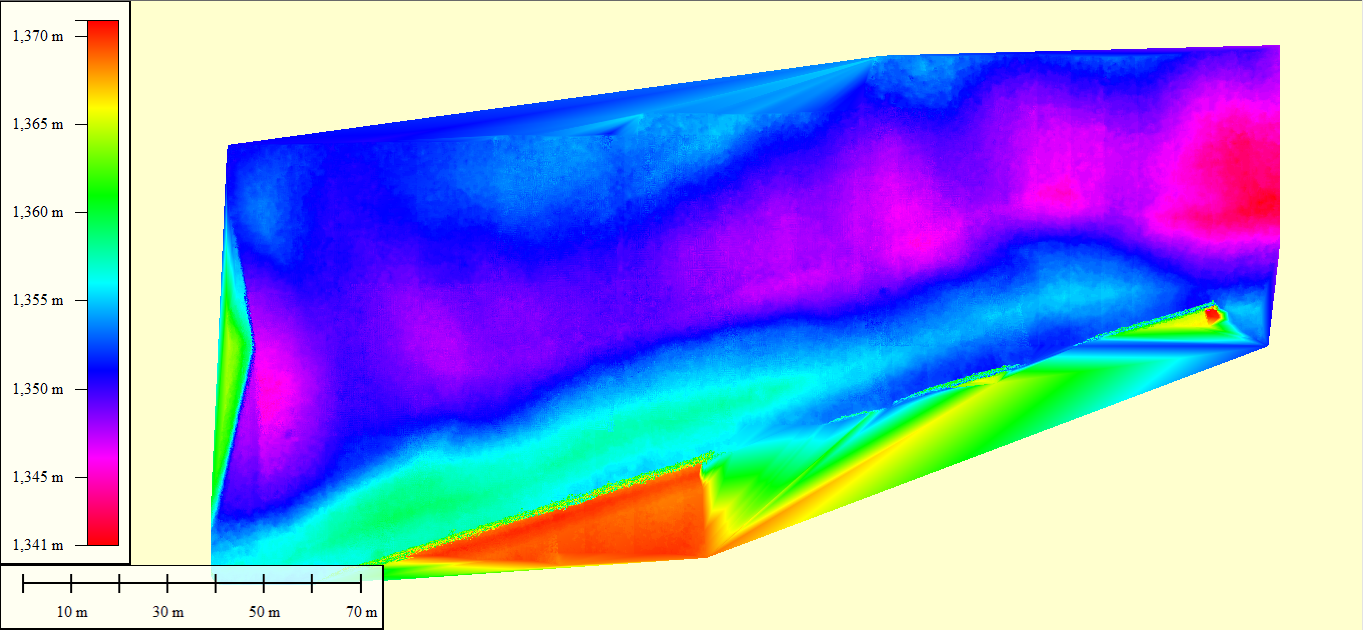
\includegraphics[width=\imsizeL]
{Q4200_dem}
\caption[DEM Ensayo 3]
{Ensayo 1. Foso de erosión aguas abajo del dique fijo. Modelo digital de elevaciones.}
\label{fig:Q4200_dem}
\end{figure}

\subsection{Medición de formas de fondo}
\label{sec:ensayo-formas-de-fondo}

Estas mediciones se realizaron con el objetivo de verificar y optimizar las consignas de operación de las estructuras de control, con el fin de regular los procesos hidrosedimentológicos presentes en las proximidades de la presa aguas arriba.\\
En este ensayo se relevaron las canalizaciones hacia las compuertas del dique móvil y el canal moderador. El análisis de los canales que se formaron sobre la superficie del modelo, debido a las llamadas que se realiza con la operación de las estructuras de control, requiere relevar una densidad de puntos elevada y a la vez cubrir grandes áreas de superficie. La técnica digital aborda esta tarea de forma mucha más eficiente y precisa que la metodología tradicional. \\
Se muestran los mapas de elevación en escala prototipo, generados a partir del área de modelación aguas arriba del dique, para el ensayo 10. Como punto de referencia se utilizó la parte superior del dique móvil, con cota igual a 1377.77 m s.n.m.

\begin{figure}[ht]
\centering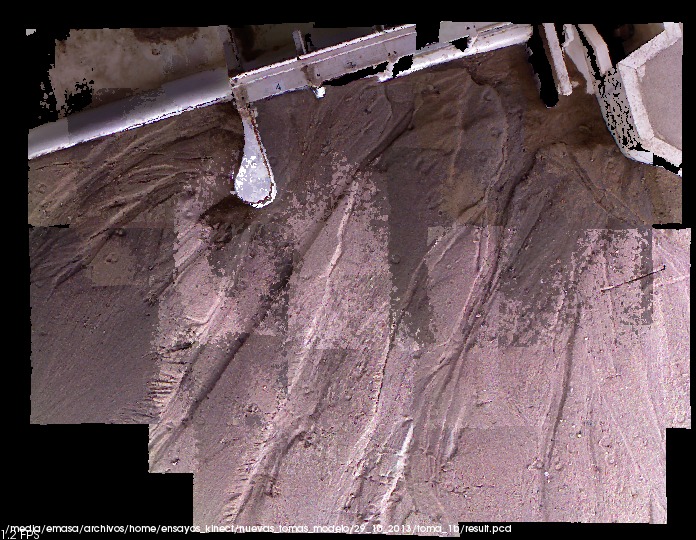
\includegraphics[width=\imsizeL]
{Q600_rgb}
\caption[Imagen RGB Ensayo 10]
{Ensayo 10. Área aguas arriba del dique móvil. Imagen RGB.}
\label{fig:Q600_rgb}
\end{figure}

\begin{figure}[ht]
\centering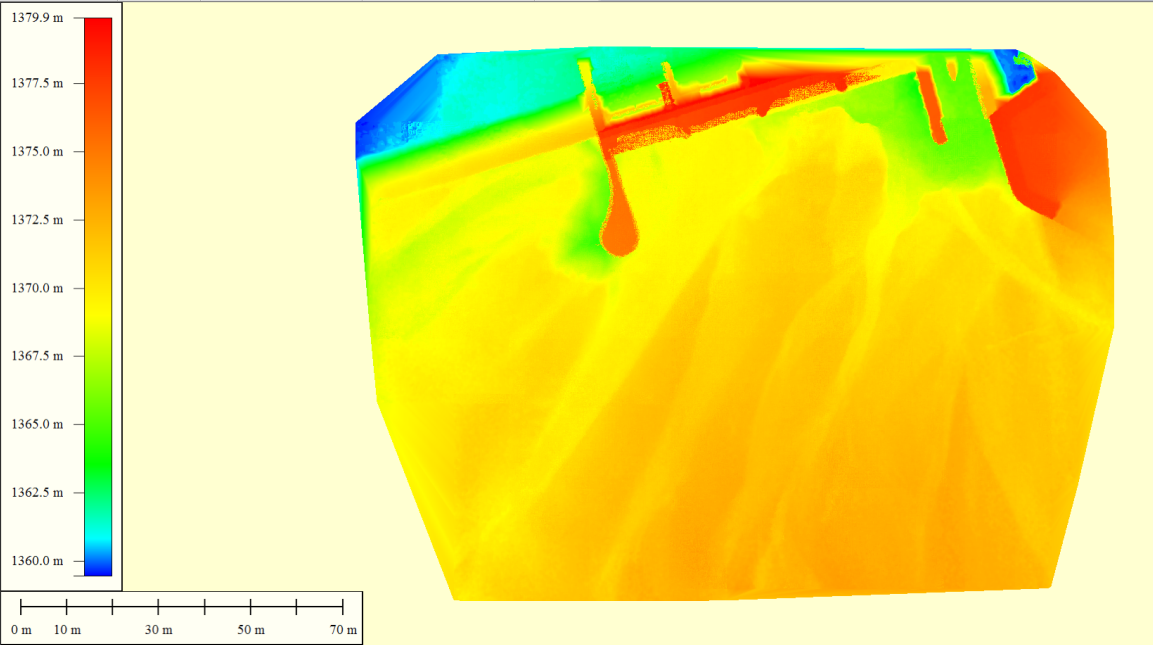
\includegraphics[width=\imsizeL]
{Q600_dem}
\caption[DEM Ensayo 10]
{Ensayo 10. Área aguas arriba del dique móvil. Modelo digital de elevaciones.}
\label{fig:Q600_dem}
\end{figure}

\chapter{Análisis de los resultados}
En este capítulo se analizan varios aspectos de la técnica digital en contraste con la técnica tradicional buscando validar la solución propuesta y demostrar las ventajas que esta presenta.

\section{Comparación de perfiles}
Utilizando los resultados presentados en los ensayos \ref{sec:ensayo-erosion-maxima}, se comparan perfiles obtenidos con ambas técnicas con el objetivo de estudiar la bondad de la técnica digital para relevar la condición de erosión. \\
En la figura \ref{fig:comparacion-perfiles}, se muestran tres perfiles sobre el foso de erosión capturados con las tecnicas digital y tradicional. \\
En el perfil superior izquierdo, se observa que los datos continuos relevados con la cámara son aproximados de forma precisa por las mediciones con nivel óptico en condiciones donde el terreno no presenta cambios abruptos. \\
En el perfil superior derecho, se observan 3 mediciones, a 30 m, 42 m y 60 m respectivamante, que se presumen haber sido tomadas de forma incorrecta con el nivel optico. No obstante, sirve para ilustrar que la tecnica tradicional puede sufrir de errores de hasta 15 mm en prototipo, o equivalentemente, 1 m en prototipo (utilizando una escala 1:65) que no podrian ser detectados sin una superficie de referencia. Aproximadamente a los 50 m se incurre en un error de una indole distinta. En este caso, la causa de la medicion incorrecta es un cambio abrupto en la condicion del terreno, que no pudo ser detectada por el operador de la mira debido la escala del modelo. \\ 
En última instancia, se presenta el perfil inferior donde se observa el efecto de la pendiente del foso de erosión sobre una serie de mediciones con nivel. En este caso, la pendiente dificulta el apoyo del palpador sobre la superficie sin producir alteraciones, derivando en mediciones por encima del valor real. \\
Estas comparaciones ponen en evidencia que la resolución del modelo 3D obtenido con la técnica digital, es superior en zonas donde los datos relevados con la técnica tradicional no han sido cuidadosamente elegidos o el terreno es muy irregular. Cuando estos errores no están presentes, la precisión de ambas técnicas se encuentra similar.

\begin{figure}[ht]
\centering
\begin{minipage}[h]{.45\textwidth}
\begin{center}
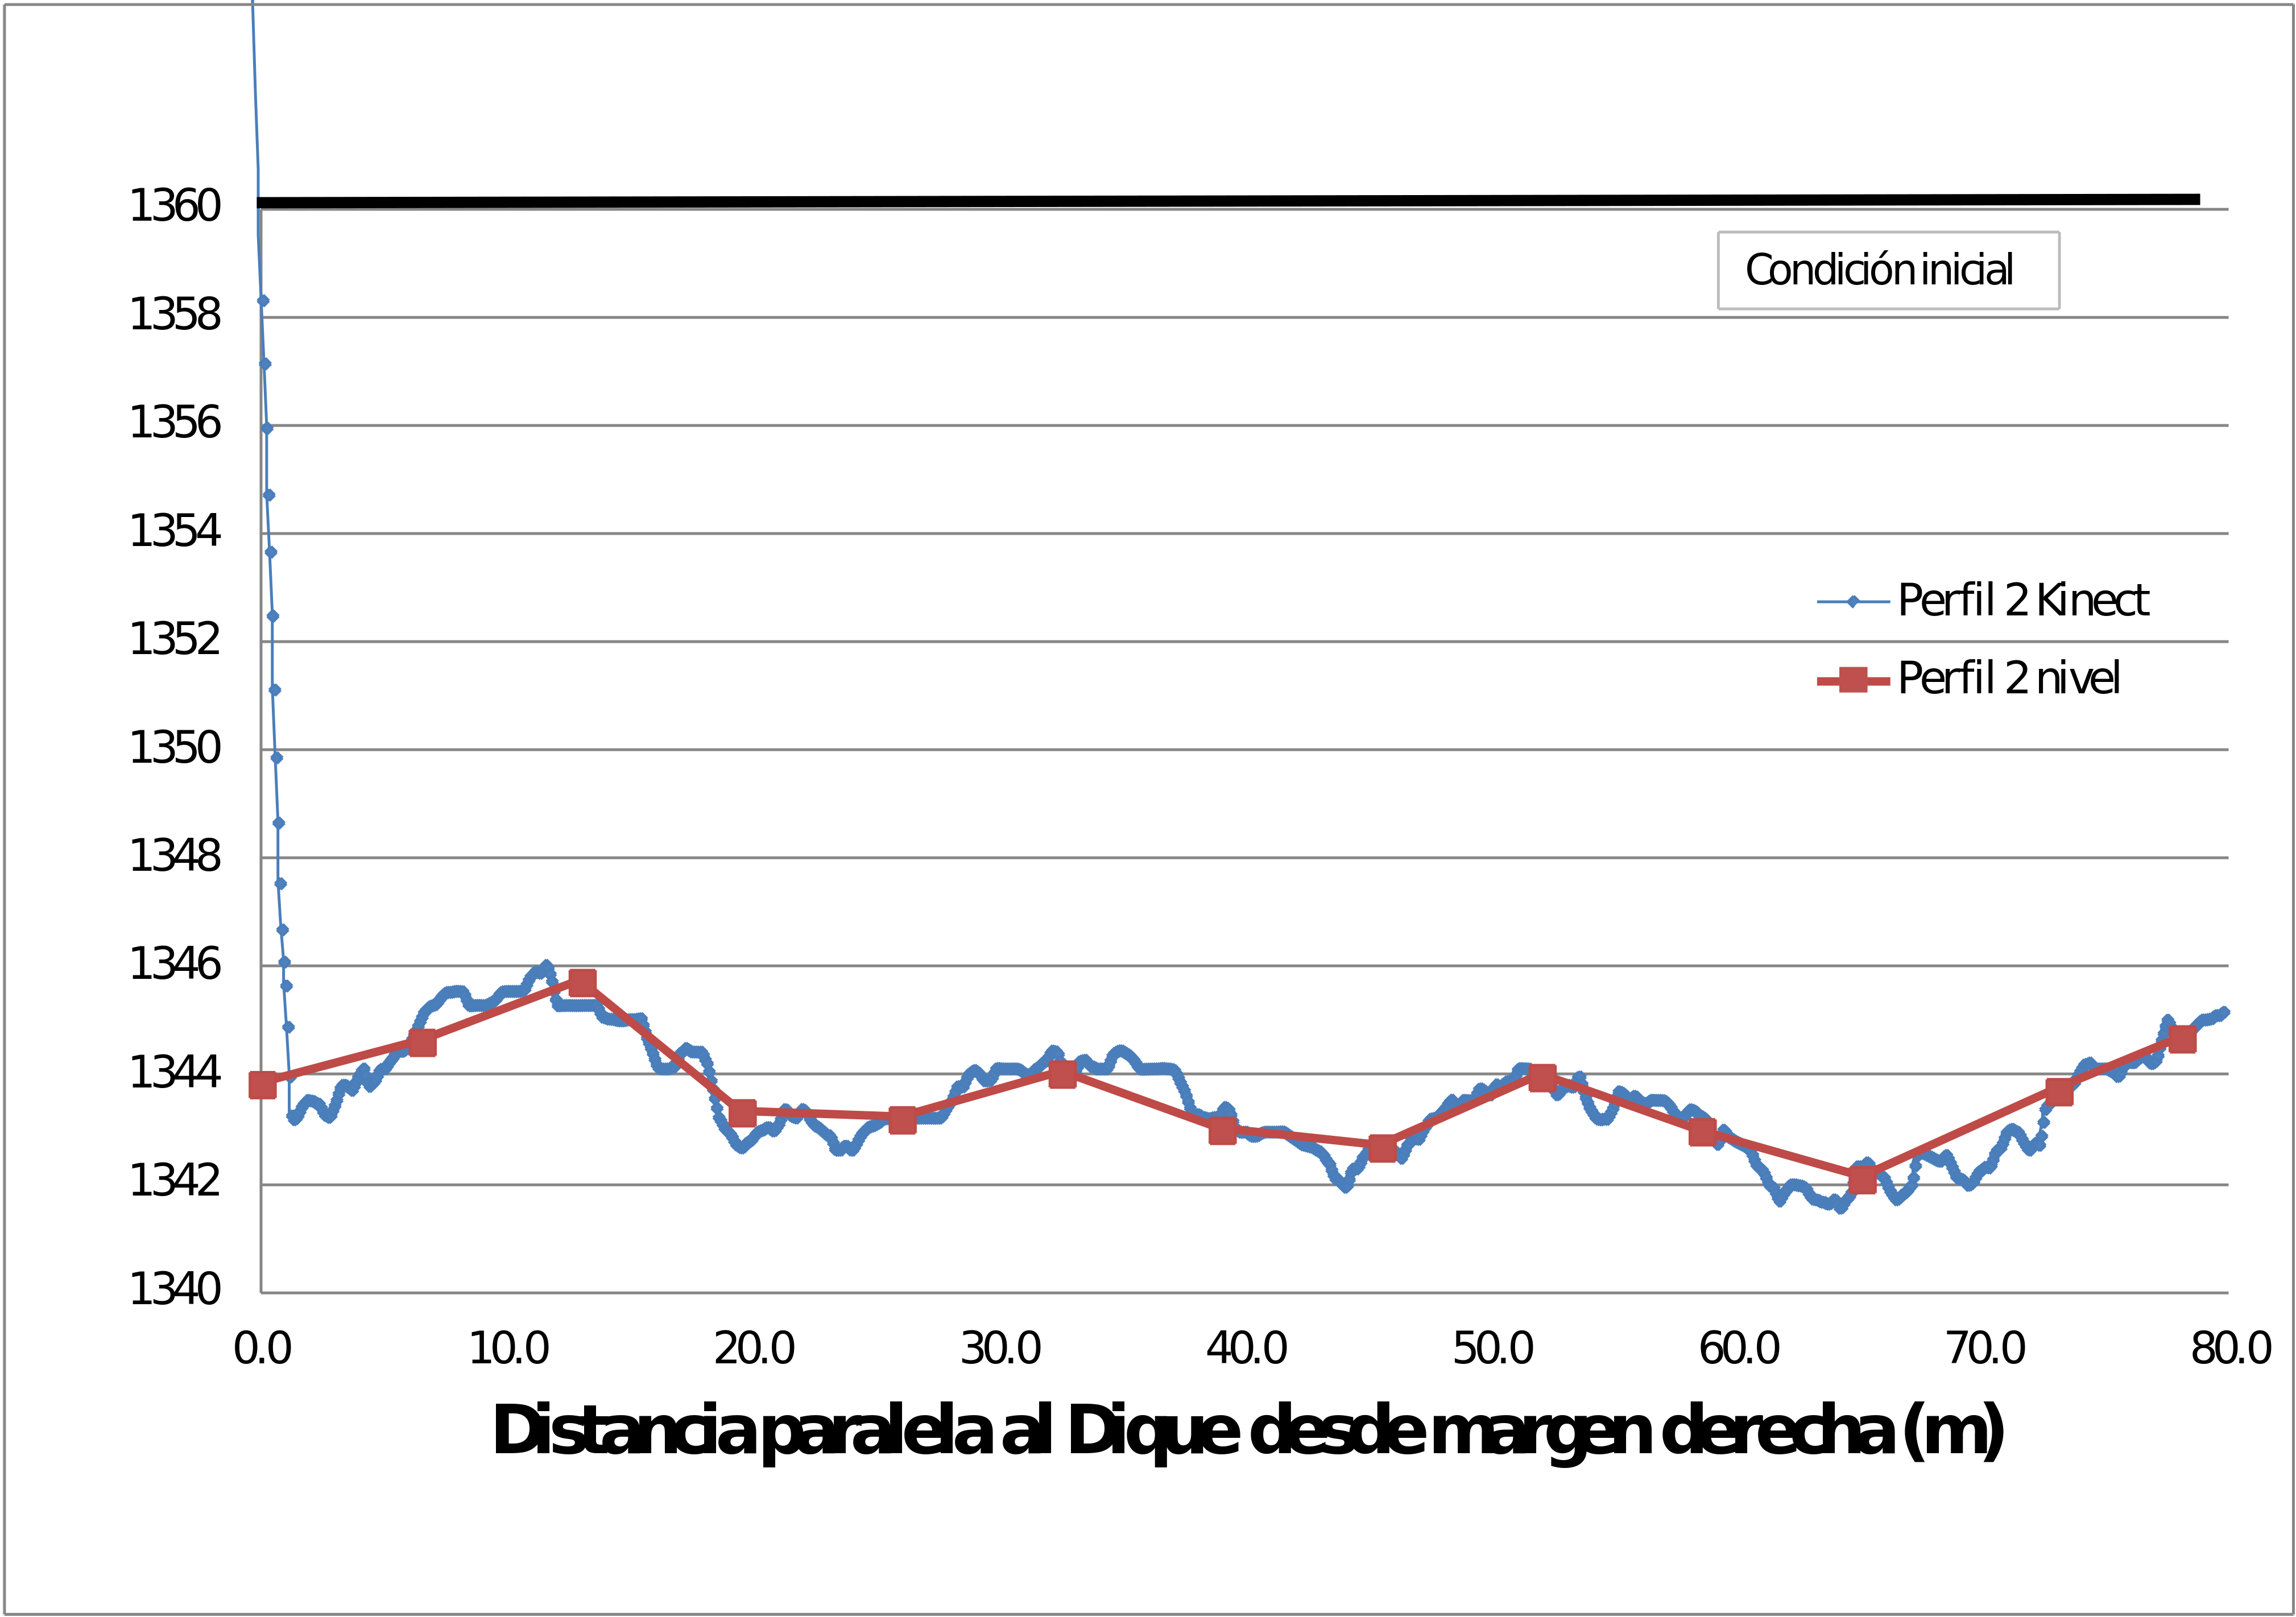
\includegraphics[width=\imsizeS]{foso-erosion-izquierda}
\end{center}
\end{minipage}
\hfill
\begin{minipage}[h]{.45\textwidth}
\begin{center}
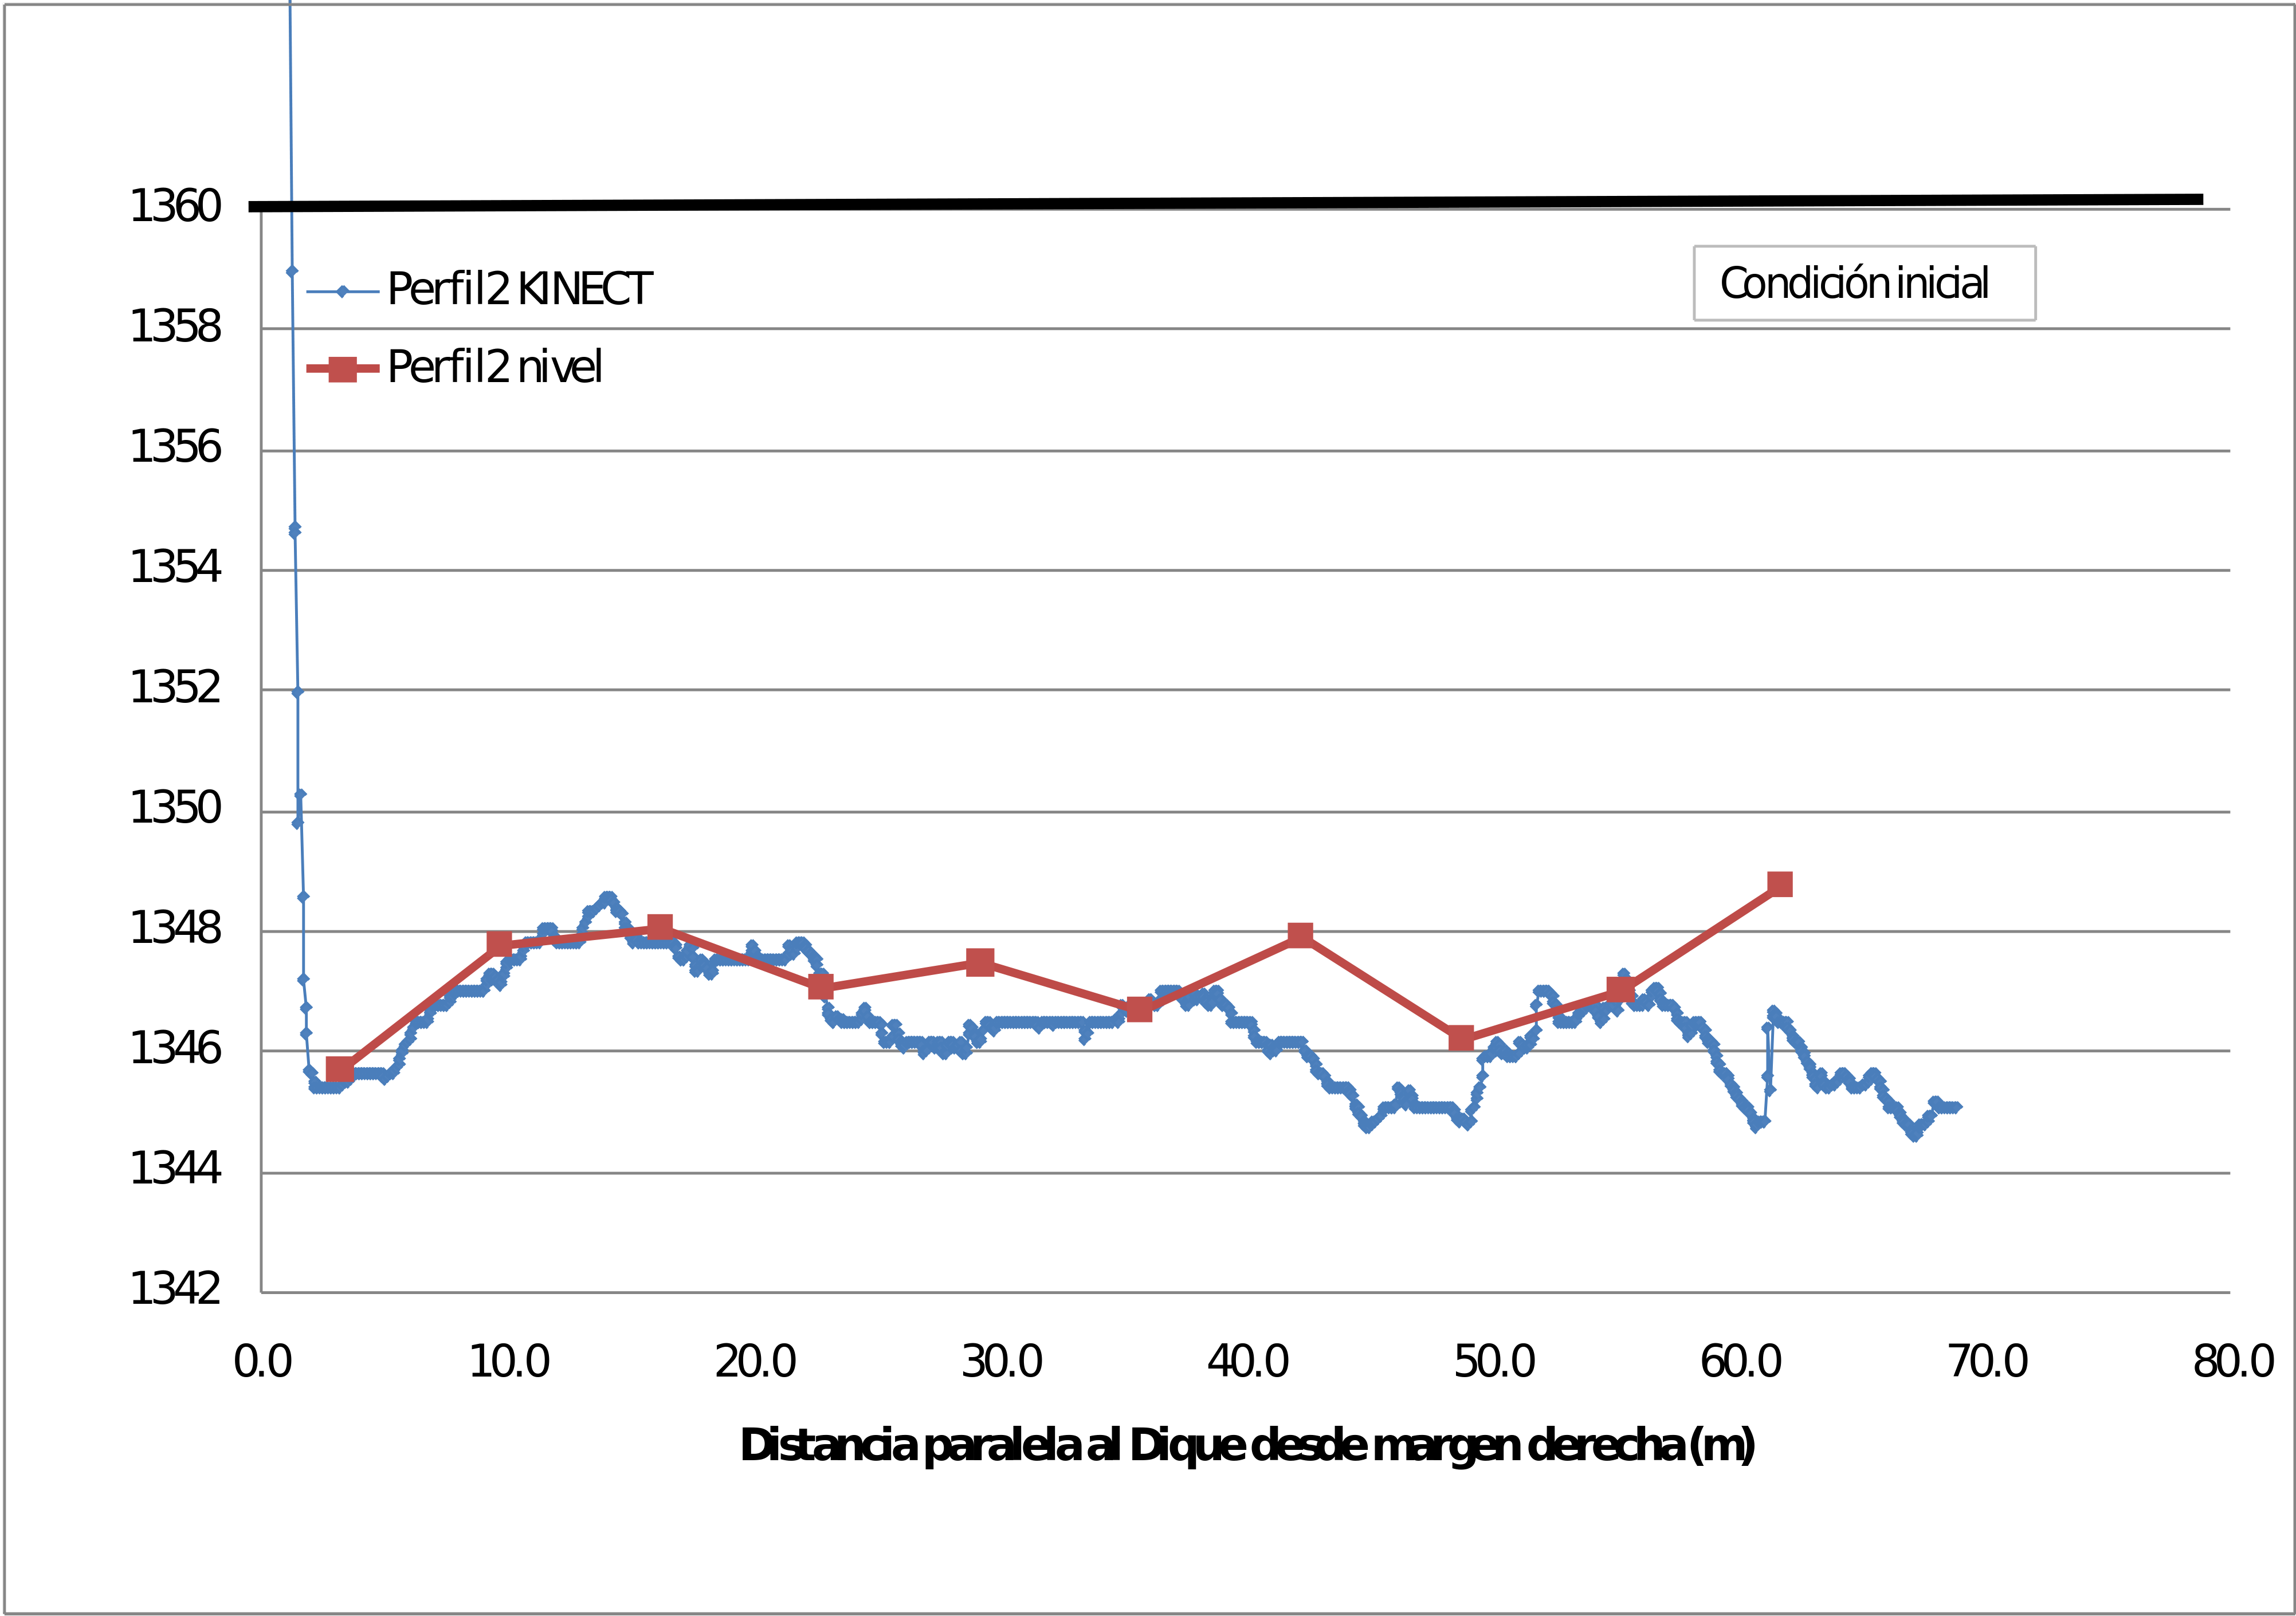
\includegraphics[width=\imsizeS]{foso-erosion-centro}
\end{center}
\end{minipage}
\hfill
\begin{minipage}[h]{.45\textwidth}
\begin{center}
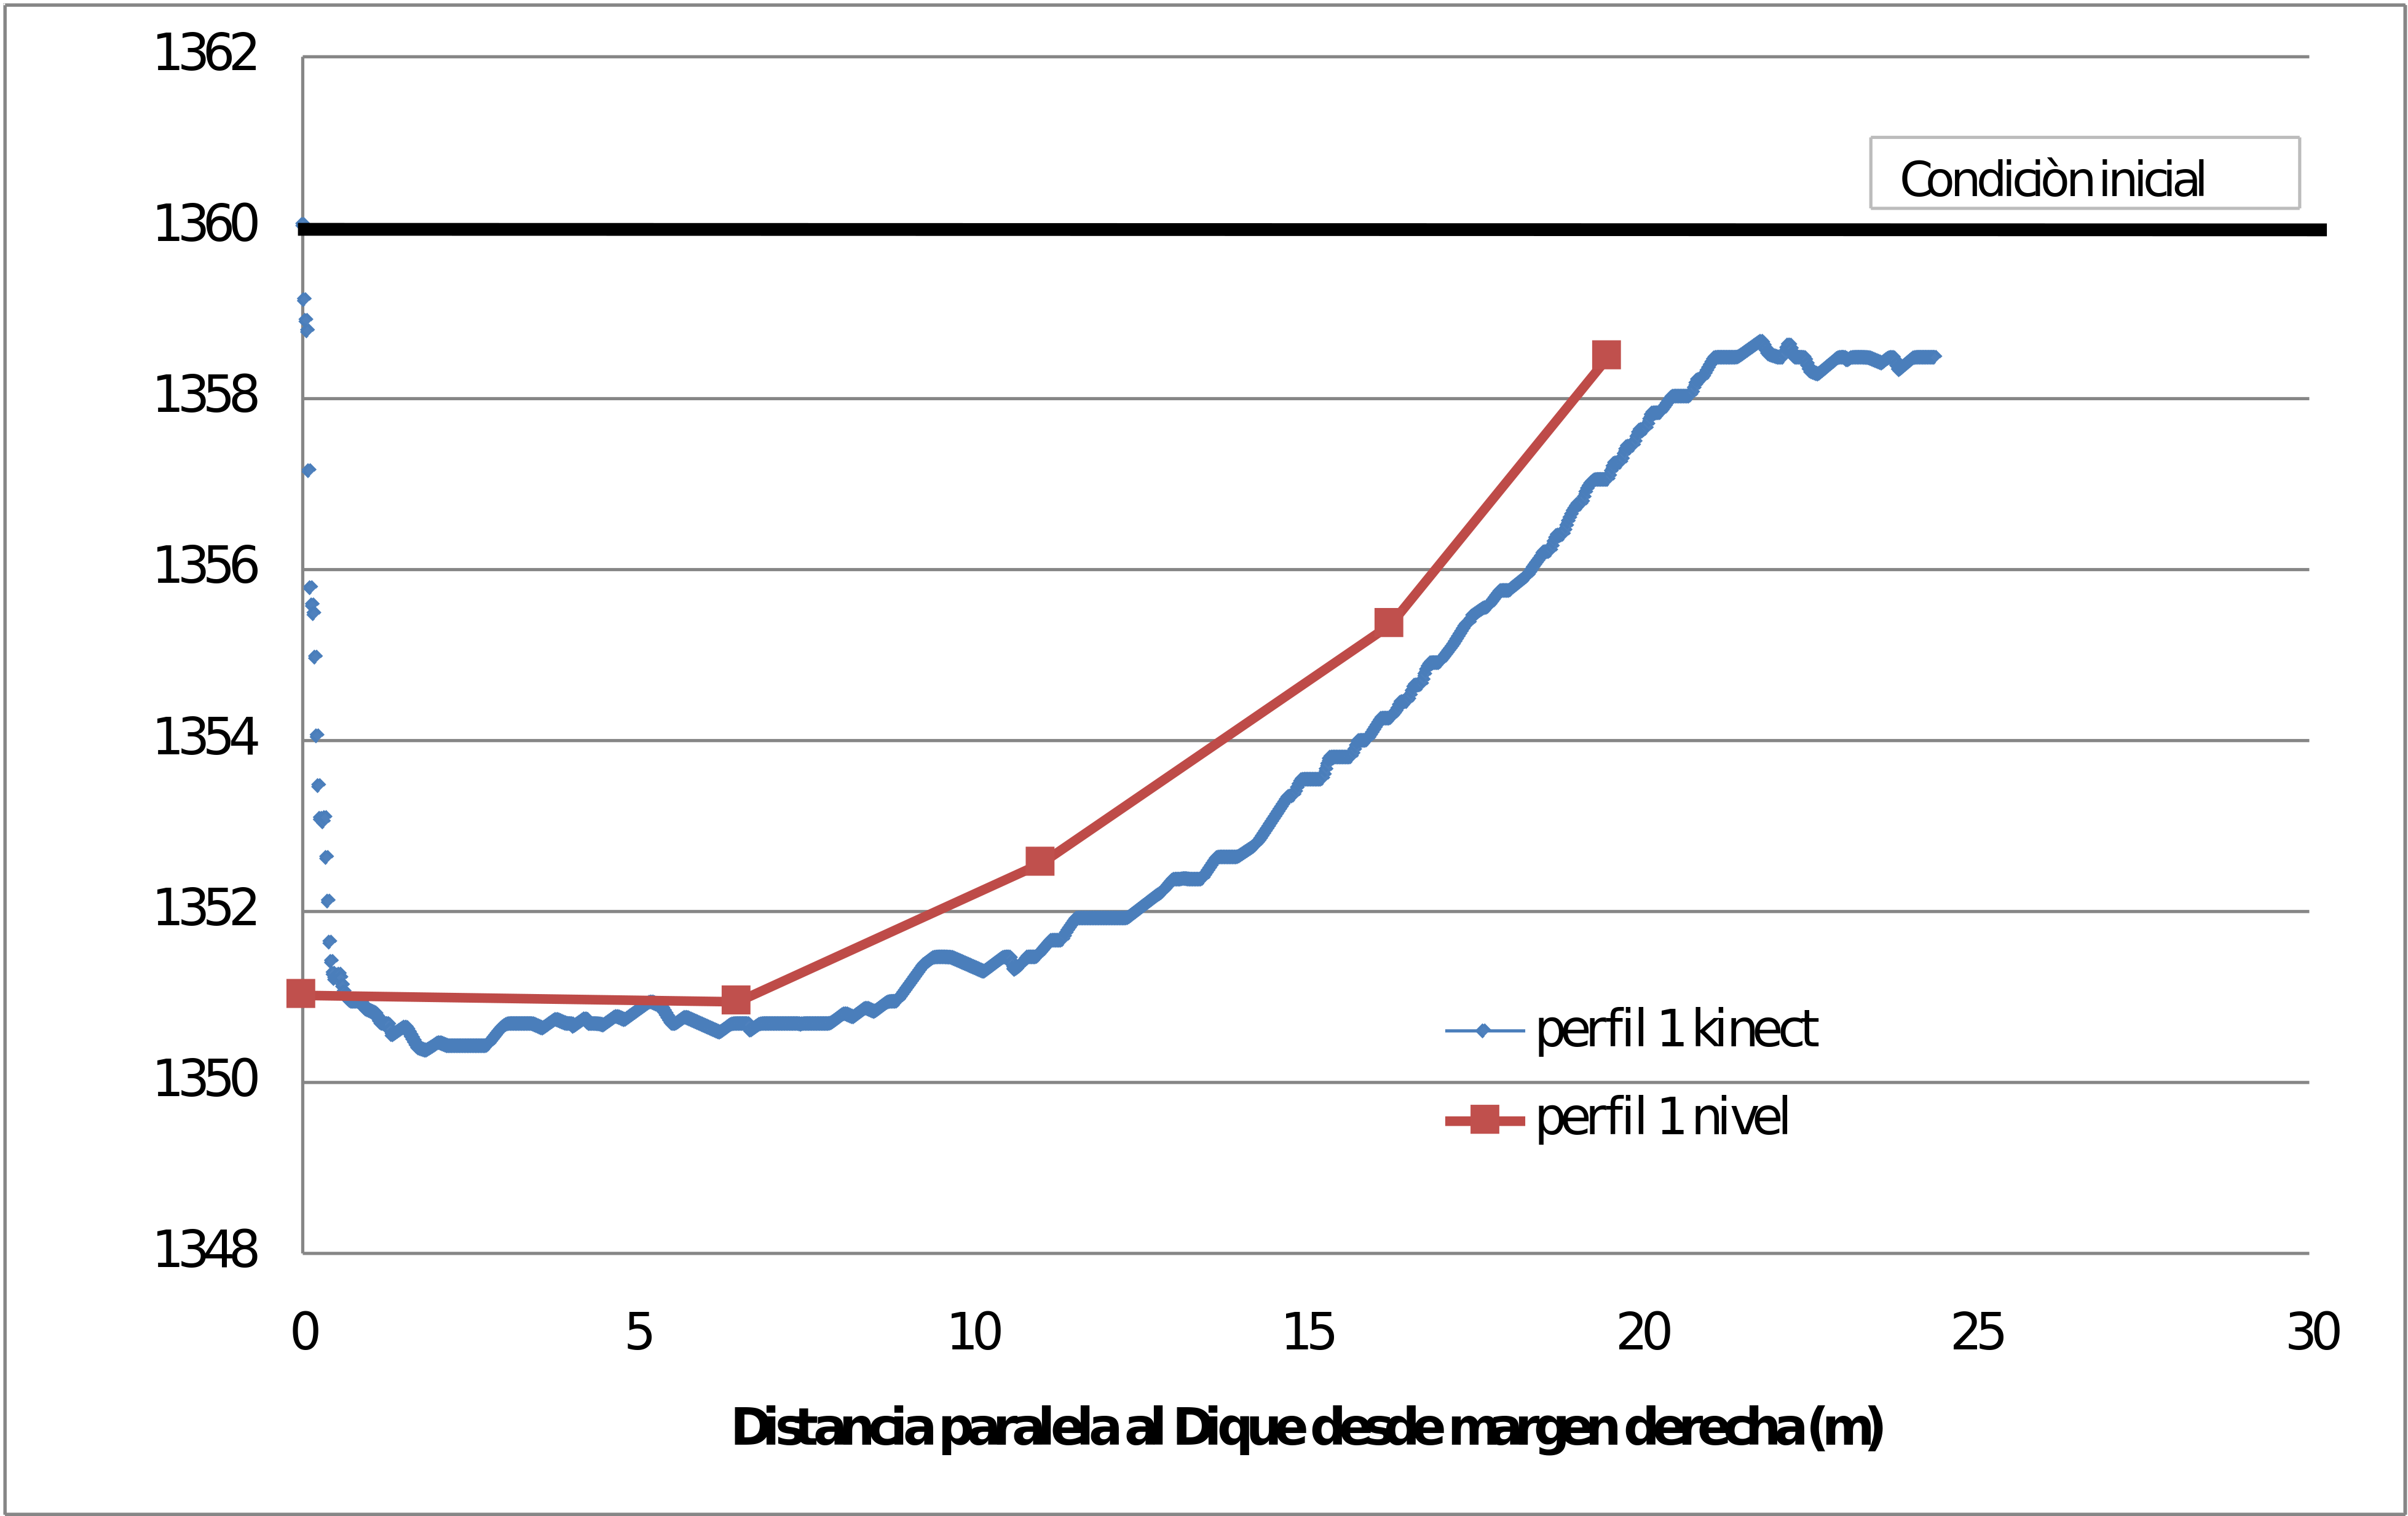
\includegraphics[width=\imsizeS]{foso-erosion-derecha}
\end{center}
\end{minipage}
\hfill
\caption[Comparación de perfiles del foso de erosión con nivel óptico y cámara Kinect]
{Comparación de perfiles del foso de erosión relevados con nivel óptico y con cámara Kinect.}
\label{fig:comparacion-perfiles}
\end{figure}

\newpage % Salto de página para acomodar las imágenes

\section{Erosión máxima}
A continuación se presentan las máximas erupciones observadas en el foso de erosión aguas abajo del canal moderador y el dique móvil relevando tanto con nivel y mira como con la cámara RGB-D.

\begin {table}[H]
\caption {Máximos niveles de erosión en el Canal Moderador} 
\label{tab:erosion-maxima-cm} 
\begin{center}

\begin{tabular}{|c|c|c|c|c|c|}
\hline 
Caudal $m^{3}/s$&Ensayo&Nivel óptico (m)&Kinect (m)&Diferencias &Diferencias\\
                &      &                &          &absolutas en &absolutas en\\
                &      &                &          &prototipo (m)&modelo (mm)\\ 
\hline 
90 & 4 & 1350.96 & 1350.37 & 0.59 & 9.07\\ 
\hline 
600 & 14 & 1349.5 & 1349.16 & 0.34 & 5.23 \\ 
\hline 
900 & 1 & 1344.8 & 1345.75 & 0.95 & 14.61\\ 
\hline 
1600 & 13 & 1345.7 & 1345.38 & \textbf{0.32} & \textbf{4.92}\\
\hline
4200 & 7 & 1345.2 & 1345.59 & 0.39 & 6\\ 
\hline 
4200 & 9 & \textbf{1344.6} & \textbf{1344.18} & 0.42 & 6.46 \\ 
\hline 
     &   &        & Promedio & 0.501 & 7.71 \\    
\hline 
     &   &        & Desv. estándar & 0.218 & 3.36 \\
\hline 
\end{tabular}
\end{center}
\end{table}

\begin {table}[H]
\caption {Máximos niveles de erosión en el Dique Móvil} 
\label{tab:erosion-maxima-dm}
\begin{center}
 
\begin{tabular}{|c|c|c|c|c|c|}
\hline 
Caudal $m^{3}/s$&Ensayo&Nivel óptico (m)&Kinect (m)&Diferencias &Diferencias\\
                &      &                &          &absolutas en &absolutas en\\
                &      &                &          &prototipo (m)&modelo (mm)\\ 
\hline 
220 & 5 & 1354.2 & 1354.89 & 0.69 & 10.61 \\ 
\hline 
600 & 14 & 1350.1 & 1349.67 & 0.43 & 6.61 \\   
\hline 
900 & 1 & 1346.1 & 1345.86 & 0.24 & 3.69 \\ 
\hline 
4200 & 7 & \textbf{1342.3} & \textbf{1343.2} & 0.9 & 13.84 \\  
\hline 
4200 & 9 & 1343.2 & 1343.41 & \textbf{0.21} & \textbf{3.23} \\
\hline 
     &   &        & Promedio & 0.493 & 7.6 \\
\hline 
     &   &        & Desv. estándar & 0.265 & 4.08 \\
\hline 
\end{tabular}
\end{center}
\end{table}

\begin{figure}[ht]
\centering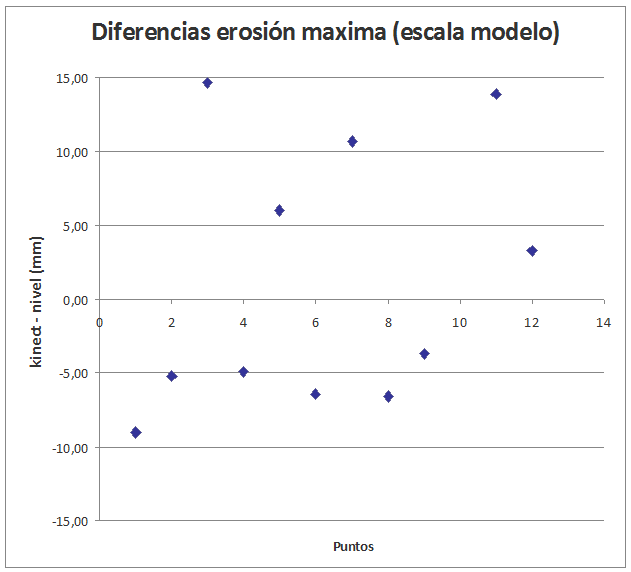
\includegraphics[width=\imsizeS]
{diferencias-erosion-maxima-modelo}
\caption[Diferencias entre mediciones de erosión máxima Kinect y Nivel]
{Diferencias (con signo) entre mediciones de erosión máxima relevadas con Kinect y con nivel óptico (en escala modelo).}
\label{fig:diferencias-erosion-maxima-modelo}
\end{figure}

Se observó un promedio en las diferencias absolutas de 7.7 mm aproximadamente y una desviación estándar de hasta 4 mm. Teniendo en cuenta que la técnica tradicional contempla errores de hasta 15 mm y el error asociado al sensor de profundidad de la Kinect es de hasta 5 mm, se considera que las mediciones realizadas con la tecnica digital estan dentro del rango aceptable para ensayos de erosión máxima. \\
Se llevó a cabo un análisis de regresión lineal simple (correlación) entre las mediciones realizadas con ambas técnicas (en escala prototipo) y se obtuvo un coeficiente de correlación $R^{2} = 0.976$, mostrando efectivamente que las mediciones entre ambas técnicas están altamente correlacionadas.

\begin{figure}[ht]
\centering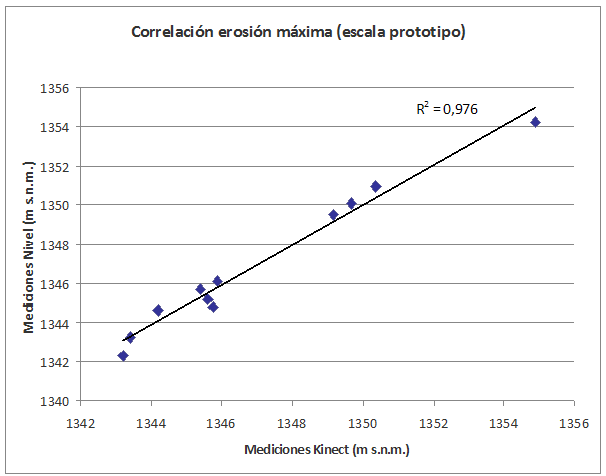
\includegraphics[width=\imsizeS]
{correlacion-erosion-maxima-prototipo}
\caption[Análisis de correlación entre mediciones de erosión máxima Kinect y Nivel]
{Análisis de correlación entre mediciones de erosión máxima Kinect y Nivel en escala prototipo. Se obtiene un $R^{2} = 0.976$.}
\label{fig:correlacion-erosion-maxima-prototipo}
\end{figure}

\section{Relevamiento de canalizaciones}

En este apartado se estudia las bondades que presenta la técnica digital para relevar el modelo físico con precisión global y se realizaron una comparación con respecto a los resultados derivados de aplicar la técnica tradicional. \\
En la sección \ref{sec:ensayo-formas-de-fondo} se presentan los resultados obtenidos para uno de los ensayos hidráulicos realizados que estudia formas de fondo generadas aguas arriba del dique para un caudal de $600 m^{3}/s$. \\
La problemática asociada a este tipo de estudios radica en la necesidad de relevar áreas extensas y con alta densidad de puntos. relevando puntos equidistantes sobre varios perfiles transversales y añadiendo la medición de puntos extras que se consideran representativos en la definición de las canalizaciones resultantes. Para obtener una aproximación global de las canalizaciones se debe generar un modelo 3D utilizando metodos de interpolacion \cite{wiki-interpolacion}.

\begin{figure}[ht]
\centering
\begin{minipage}[h]{.45\textwidth}
\begin{center}
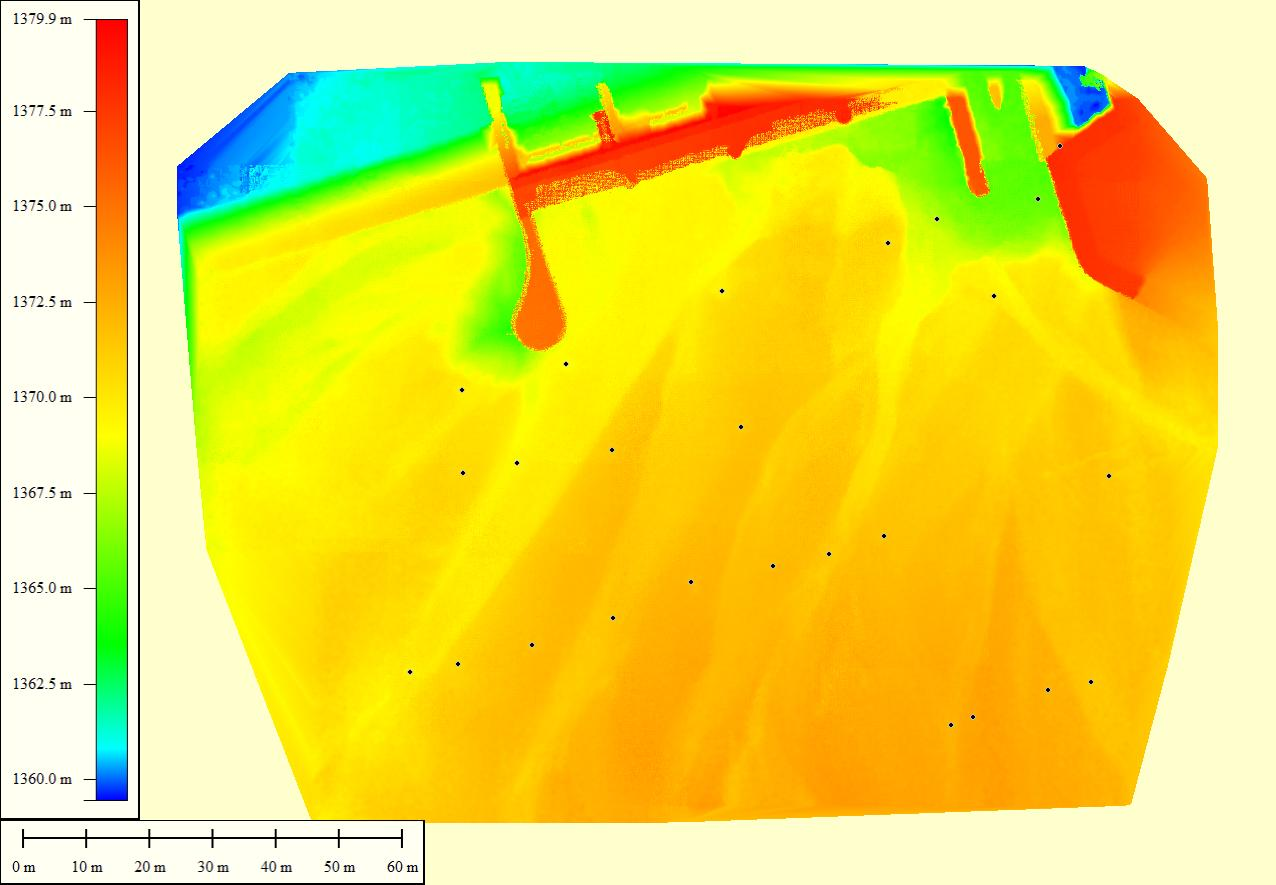
\includegraphics[width=\imsizeS]{dem-kinect}
\end{center}
\end{minipage}
\hfill
\begin{minipage}[h]{.45\textwidth}
\begin{center}
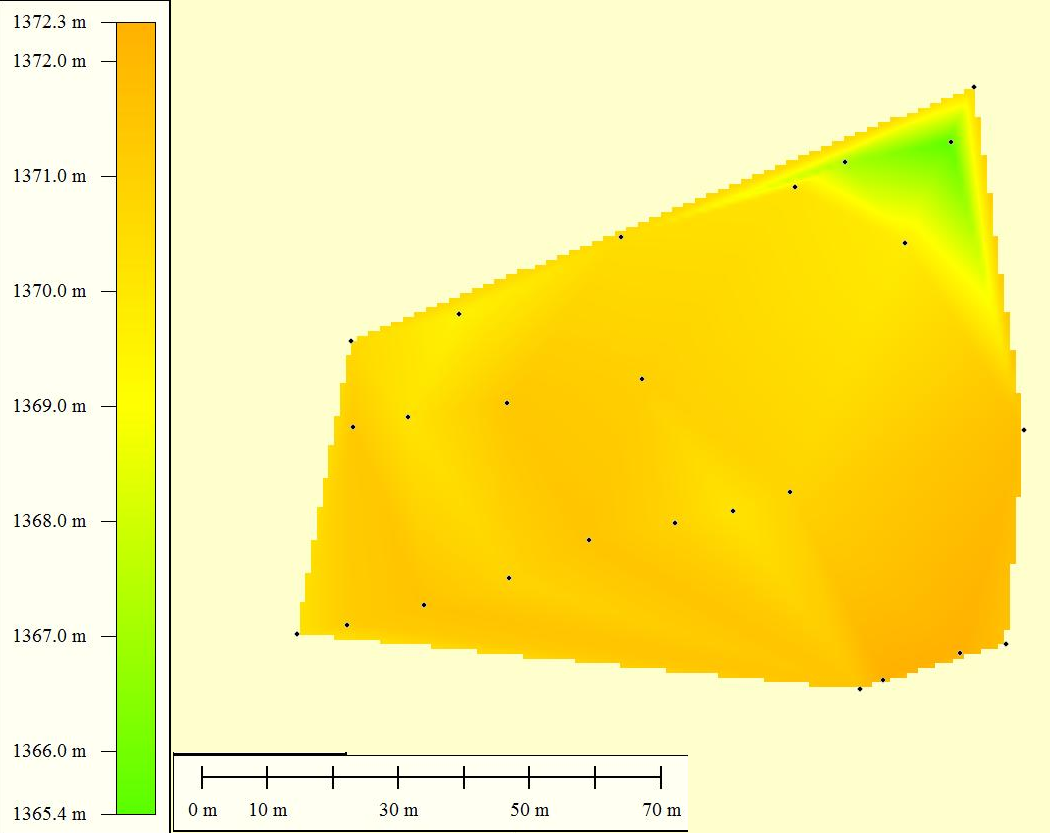
\includegraphics[width=.95\textwidth]{dem-interpolacion-nivel}
\end{center}
\end{minipage}
\hfill
\caption[DEM obtenido con Kinect y DEM generado por interpolación]
{Izquierda: DEM relevado por el sensor Kinect. Derecha: DEM generado utilizando interpolación a partir de los puntos medidos con nivel óptico. Se superponen las mediciones con nivel sobre ambos DEM's a modo ilustrativo.}
\label{fig:comparacion-dem-kinect-interpolacion}
\end{figure}

En la figura \ref{fig:comparacion-dem-kinect-interpolacion} se presentan la superficie generada por medio de interpolación a partir de puntos medidos con nivel óptico (derecha) y el modelo 3D relevado con la Kinect (izquierda) sobre la misma zona. \\
Con el objetivo de analizar la fidelidad de esta aproximacion, se trazaron un par de perfiles (sobre la misma zona), uno por cada superficie, y se calcularon las diferencias entre los resultados obtenidos con la tecnica digital y los derivados de la tecnica tradicional. En la figura \ref{fig:perfiles-diferencia-kinect-interpolacion} se presenta este experimento para cuatro cortes distintos. Se pueden apreciar zonas con diferencias de mediciones (con respecto a los valores en prototipo) dentro del intervalo $\pm0,5$ m. Este intervalo representa en modelo $\pm 7,69$ mm, lo que se considera aceptable en cuanto a la precisión de mediciones longitudinales intrusivas que se pueden alcanzar en modelos físicos. No obstante, este analisis muestra que existen dentro de estas extensas áreas relevadas, zonas donde las canalizaciones relevadas con la tecnica digital tienden a estar ubicadas entre $0,5$ m a $1,5$ m (en escala prototipo) por debajo de las canalizaciones aproximadas. Estos resultados derivan del hecho que la precision asociada a metodos de interpolacion disminuye cuando la funcion se aleja de las mediciones reales. \\
La discrepancia entre los distintos modelos 3D es demasiado alta, lo que refleja que la aproximación por interpolación no representa de forma precisa la condición real . \\
Cabe recalcar, que se puede disminuir el error presente en la superficie aproximada incrementando la cantidad de puntos relevados con la técnica tradicional (nivel y mira). Sin embargo, es simple inducir que la tecnica tradicional implica mayor tiempo de medición para relevar areas extensas con la densidad de puntos necesaria para estudios de formas de fondo. Y este proceso es tedioso cuando se deben realizar ensayos consecutivos y secuenciales asociados a aspectos complementarios del estudio global. En vista de lo anterior, se concluye que el enfoque propuesto en este trabajo permite obtener una fiel caracterizacion de las canalizaciones con un bajo costo-tiempo de medicion, resolviendo asi la problematica asociada a este tipo de ensayos. \\

\begin{figure}[ht]
\centering
\begin{minipage}[h]{.45\textwidth}
\begin{center}
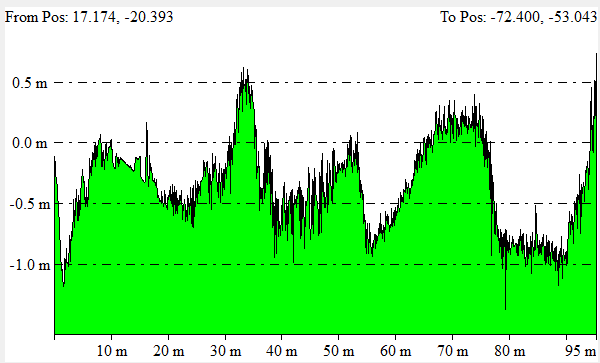
\includegraphics[width=.92\textwidth]{perfil-diferencias-kinect-interpolacion-1}
\end{center}
\end{minipage}
\hfill
\begin{minipage}[h]{.45\textwidth}
\begin{center}
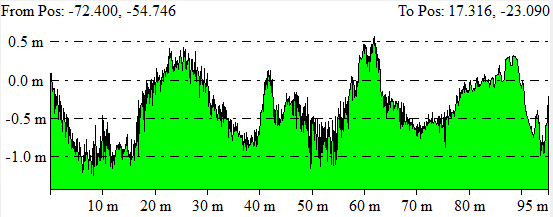
\includegraphics[width=\imsizeS]{perfil-diferencias-kinect-interpolacion-2}
\end{center}
\end{minipage}
\hfill
\begin{minipage}[h]{.45\textwidth}
\begin{center}
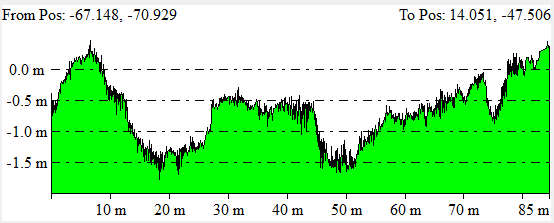
\includegraphics[width=\imsizeS]{perfil-diferencias-kinect-interpolacion-3}
\end{center}
\end{minipage}
\hfill
\begin{minipage}[h]{.45\textwidth}
\begin{center}
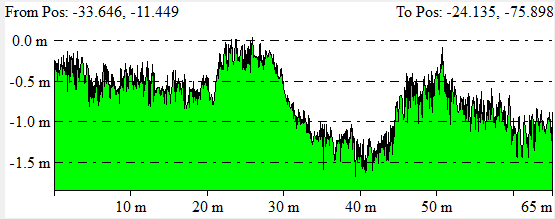
\includegraphics[width=\imsizeS]{perfil-diferencias-kinect-interpolacion-4}
\end{center}
\end{minipage}
\hfill
\caption[Diferencias entre perfiles con Kinect y perfiles extraídos desde superficie interpolada]
{Diferencias entre perfiles relevados con la técnica digital y perfiles trazados sobre una superficie interpolada a partir de mediciones con la técnica tradicional.}
\label{fig:perfiles-diferencia-kinect-interpolacion}
\end{figure}

\section{Control de estructuras del dique}

En la presente sección se analiza la precisión de la técnica propuesta para representar estructuras del dique.
En las figura \ref{fig:perfil-muro-de-encauzamiento-longitudinal}, se muestra un perfil longitudinal sobre el muro de encauzamiento. Se puede observar que la representación es precisa, conservando la forma general de la estructura, pero se advierte la presencia de algunas fluctuaciones y pequeños picos. Para analizar la magnitud del error, se trazó un perfil de menor longitud (figura \ref{fig:perfil-muro-de-encauzamiento-corto}). Se obtiene que casi todos los puntos relevados se encuentran respecto del valor 1375,1 m, el cual es la cota real de la estructura en prototipo, en el intervalo $\pm 0,3$ m (exceptuando 3 observaciones a 0,35 m, 0,4 m, 0,45 m respectivamente). Esto indica que una diferencia de 0,3 m en prototipo o equivalentemente 4.61 mm en modelo, condición que se mantiene dentro del margen esperado de 5 mm, posicionando la cámara a una distancia menor a 1,5 m (apartado \ref{sec:consideraciones-kinect}). En la figura \ref{fig:perfil-muro-de-separacion}, se traza un perfil longitudinal sobre el muro de separación del dique fijo y el canal moderador, y se obtienen valores en el intervalo 1376,27 m $\pm 0,25$ m, es decir, un error aproximado de 3,84 mm en modelo, similar a lo observado anteriormente. \\
En la figura \ref{fig:perfil-muro-de-encauzamiento-longitudinal} destacan 2 observaciones aisladas con error de aproximadamente 6 cm en escala modelo que no pudieron ser filtradas. Se propone continuar en trabajos futuros el estudio de una metodología eficaz para eliminar este tipo de \textit{outliers}. \\
Se concluye que la técnica propuesta captura con precisión aceptable las estructuras del dique, lo que habilita a poder utilizar dichas estructuras como referencias visuales en el estudio de la erosión.

\begin{figure}[ht]
\centering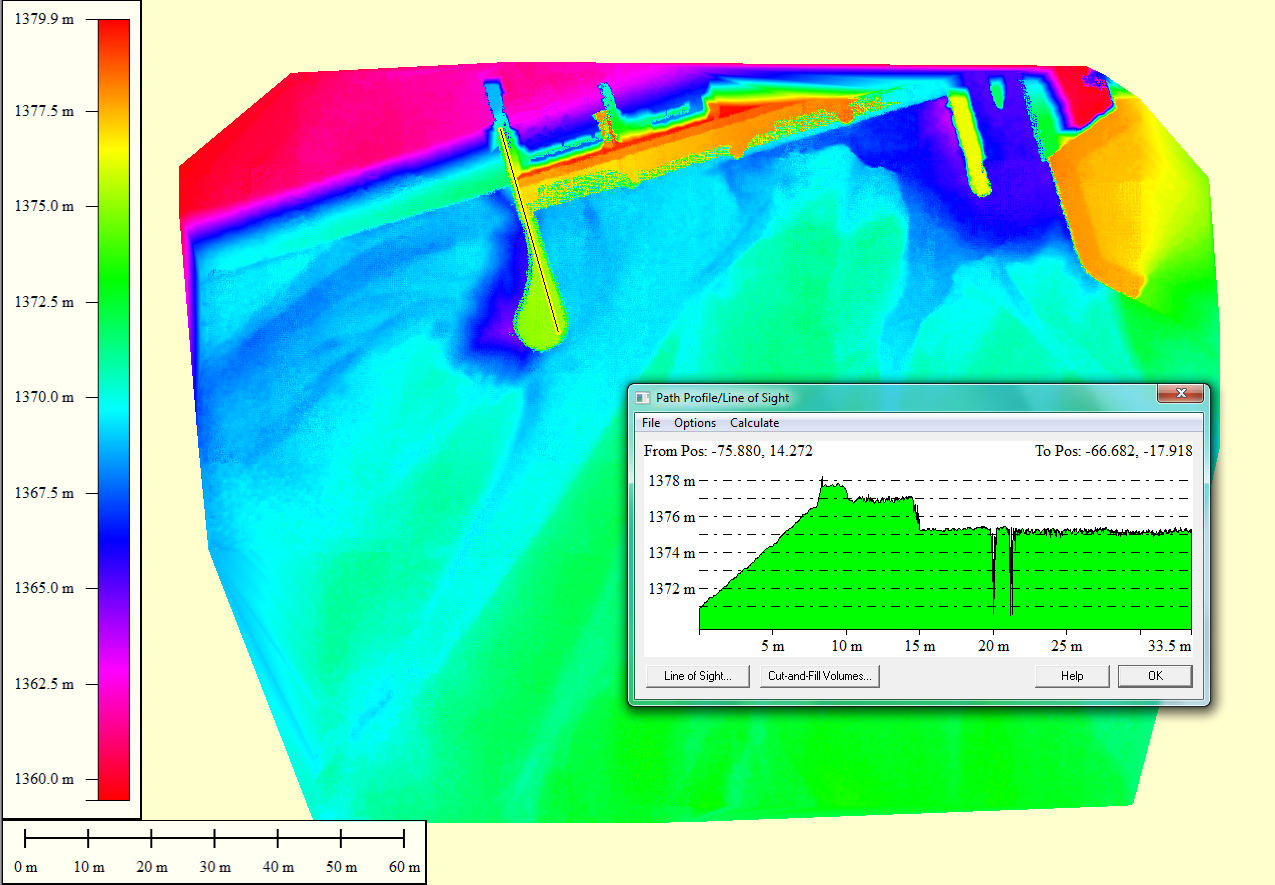
\includegraphics[width=\imsize]
{perfil-muro-de-encauzamiento-longitudinal}
\caption[Perfil longitudinal sobre el muro de encauzamiento]
{Perfil longitudinal sobre el muro de encauzamiento.}
\label{fig:perfil-muro-de-encauzamiento-longitudinal}
\end{figure}

\begin{figure}[ht]
\centering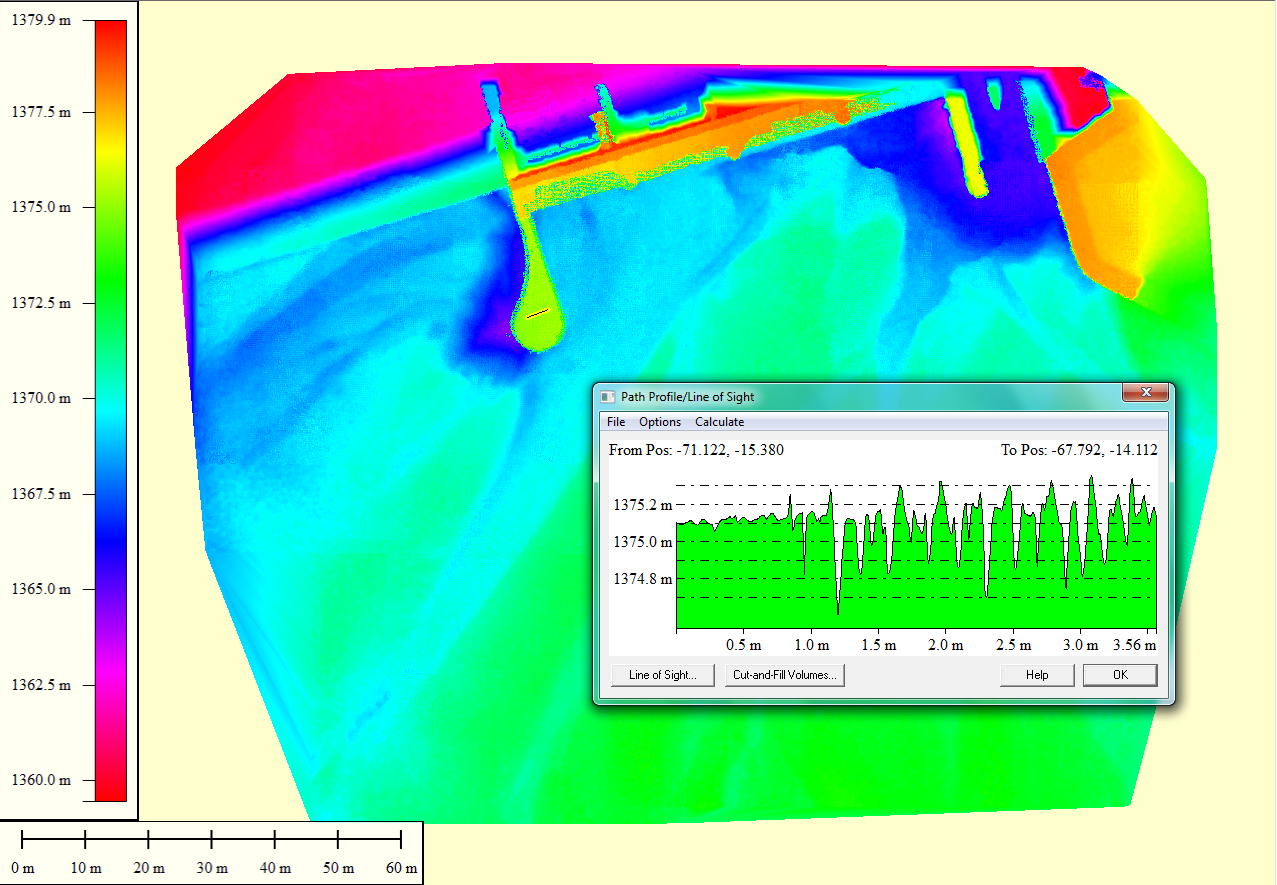
\includegraphics[width=\imsize]
{perfil-muro-de-encauzamiento-corto}
\caption[Perfil corto sobre el muro de encauzamiento]
{Perfil corto sobre el muro de encauzamiento.}
\label{fig:perfil-muro-de-encauzamiento-corto}
\end{figure}

\begin{figure}[t]
\centering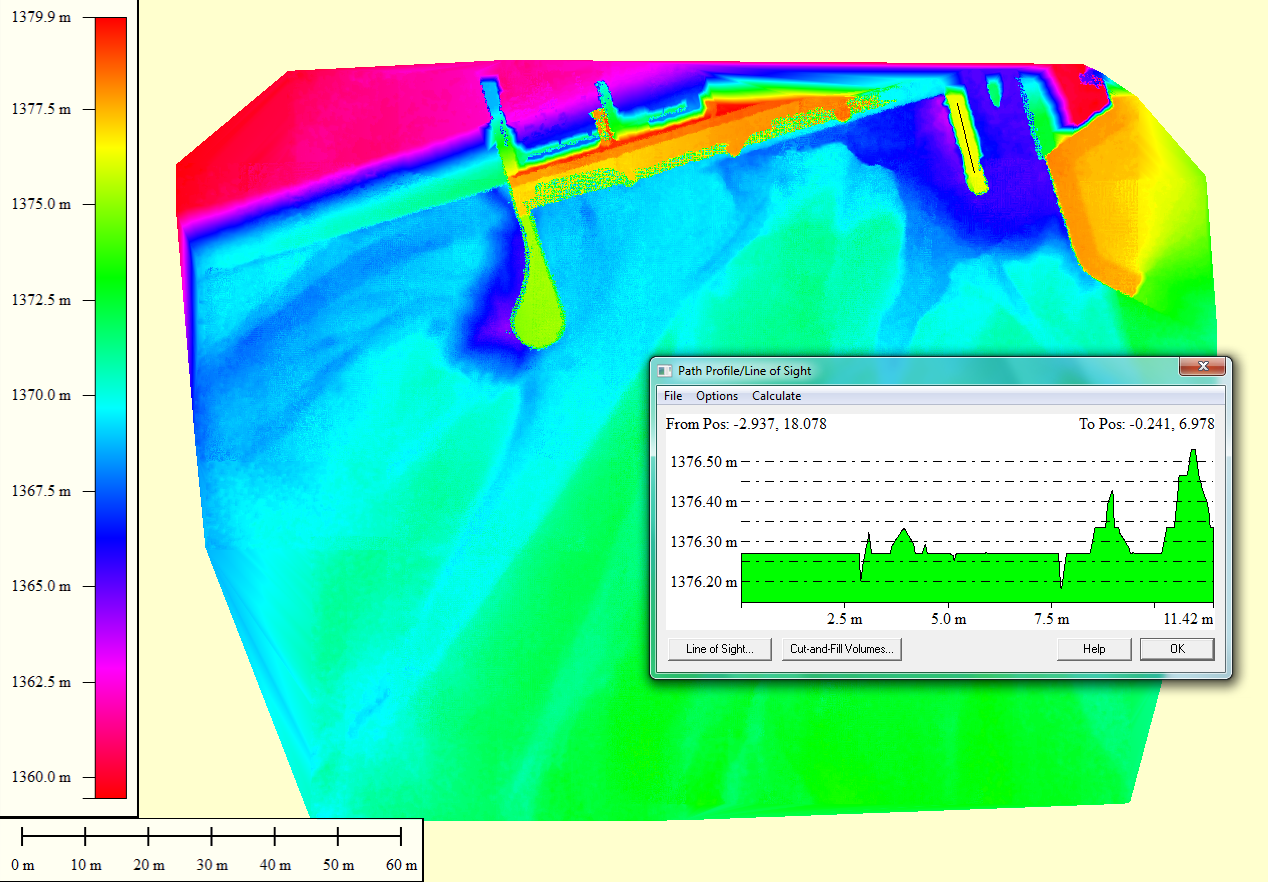
\includegraphics[width=\imsize]
{perfil-muro-de-separacion}
\caption[Perfil sobre el muro de separación entre el dique móvil y el canal moderador]
{Perfil sobre el muro de separación entre el dique móvil y el canal moderador.}
\label{fig:perfil-muro-de-separacion}
\end{figure}




\begin{biblio}
\bibliography{mibib}
\end{biblio}

\begin{postliminary}

\begin{seccion}{Publicaciones asociadas}
  \begin{enumerate}

  \item SIMPOSIO DE METODOS EXPERIMENTALES EN HIDRAULICA, SANTA FE, \textbf{2013}

  \item XXIV CONGRESO NACIONAL DEL AGUA, SAN JUAN, \textbf{2013}

  \end{enumerate}
\end{seccion}

%\begin{seccion}{Agradecimientos}
%A todos los que se lo merecen, por merecerlo
%\end{seccion}

\end{postliminary}

\end{document}